%%
%% This is file `sample-acmsmall-conf.tex',
%% generated with the docstrip utility.
%%
%% The original source files were:
%%
%% samples.dtx  (with options: `acmsmall-conf')
%% 
%% IMPORTANT NOTICE:
%% 
%% For the copyright see the source file.
%% 
%% Any modified versions of this file must be renamed
%% with new filenames distinct from sample-acmsmall-conf.tex.
%% 
%% For distribution of the original source see the terms
%% for copying and modification in the file samples.dtx.
%% 
%% This generated file may be distributed as long as the
%% original source files, as listed above, are part of the
%% same distribution. (The sources need not necessarily be
%% in the same archive or directory.)
%%
%%
%% Commands for TeXCount
%TC:macro \cite [option:text,text]
%TC:macro \citep [option:text,text]
%TC:macro \citet [option:text,text]
%TC:envir table 0 1
%TC:envir table* 0 1
%TC:envir tabular [ignore] word
%TC:envir displaymath 0 word
%TC:envir math 0 word
%TC:envir comment 0 0
%%
%%
%% The first command in your LaTeX source must be the \documentclass
%% command.
%%
%% For submission and review of your manuscript please change the
%% command to \documentclass[manuscript, screen, review]{acmart}.
%%
%% When submitting camera ready or to TAPS, please change the command
%% to \documentclass[sigconf]{acmart} or whichever template is required
%% for your publication.
%%
%%
\documentclass[manuscript,acmsmall,anonymous,review,screen,nonacm=true, authorversion=true]{acmart}

%%
%% \BibTeX command to typeset BibTeX logo in the docs
\AtBeginDocument{%
  \providecommand\BibTeX{{%
    Bib\TeX}}}

%% Rights management information.  This information is sent to you
%% when you complete the rights form.  These commands have SAMPLE
%% values in them; it is your responsibility as an author to replace
%% the commands and values with those provided to you when you
%% complete the rights form.
\setcopyright{acmcopyright}
\copyrightyear{2018}
\acmYear{2018}
\acmDOI{XXXXXXX.XXXXXXX}

%% These commands are for a PROCEEDINGS abstract or paper.
\acmConference[Conference acronym 'XX]{Make sure to enter the correct
  conference title from your rights confirmation emai}{June 03--05,
  2018}{Woodstock, NY}
%%
%%  Uncomment \acmBooktitle if the title of the proceedings is different
%%  from ``Proceedings of ...''!
%%
%%\acmBooktitle{Woodstock '18: ACM Symposium on Neural Gaze Detection,
%%  June 03--05, 2018, Woodstock, NY}
\acmPrice{15.00}
\acmISBN{978-1-4503-XXXX-X/18/06}


%%
%% Submission ID.
%% Use this when submitting an article to a sponsored event. You'll
%% receive a unique submission ID from the organizers
%% of the event, and this ID should be used as the parameter to this command.
%%\acmSubmissionID{123-A56-BU3}

%%
%% For managing citations, it is recommended to use bibliography
%% files in BibTeX format.
%%
%% You can then either use BibTeX with the ACM-Reference-Format style,
%% or BibLaTeX with the acmnumeric or acmauthoryear sytles, that include
%% support for advanced citation of software artefact from the
%% biblatex-software package, also separately available on CTAN.
%%
%% Look at the sample-*-biblatex.tex files for templates showcasing
%% the biblatex styles.
%%

%%
%% The majority of ACM publications use numbered citations and
%% references.  The command \citestyle{authoryear} switches to the
%% "author year" style.
%%
%% If you are preparing content for an event
%% sponsored by ACM SIGGRAPH, you must use the "author year" style of
%% citations and references.
%% Uncommenting
%% the next command will enable that style.
%%\citestyle{acmauthoryear}
\usepackage{booktabs}   %% For formal tables:
                        %% http://ctan.org/pkg/booktabs
\usepackage{subcaption} %% For complex figures with subfigures/subcaptions
                        %% http://ctan.org/pkg/subcaption

%%%%%%%%%%%%%%%%%%%%%%%%%%%% INPUTTING SELF DEFINED COMMANDS, SELF IMPORTED PACKAGES %%%%%%%%%%%%%%%%%%%%%%%%%%%%%%%%%%%%%%%%%%
%%%%%%%%%%%%%%%%%%%%%%%%%%%%%%%%%%%%%%%%%%%%%%%%%%%%%%%%%%%%%%%%%%%%%%%%%%%%%%%%%%%%%%%%%%%%%%%%%%%%%%%%%%%%%%%%%%%%%%%%%%%%%%%%%%%%%%%%%
%%%%%%%%%%%%%%%%%%%%%%%%%%%%%%%%%%%%%%%%%%%%%%%%%%%%% COMMANDS FOR GENERAL PAPER WRITING %%%%%%%%%%%%%%%%%%%%%%%%%%%%%%%%%%%%%%%%%%%%%%%%%%%%
%%%%%%%%%%%%%%%%%%%%%%%%%%%%%%%%%%%%%%%%%%%%%%%%%%%%%%%%%%%%%%%%%%%%%%%%%%%%%%%%%%%%%%%%%%%%%%%%%%%%%%%%%%%%%%%%%%%%%%%%%%%%%%%%%%%%%%%%%

%%%%%%%%%%%%%%%%%% LINK STYLE:
\hypersetup{
  colorlinks=true,
  linkcolor=blue!50!red,
  urlcolor=green!70!black
}

%%%%%%%%%%%%%%%%%%%%%%%%%%%% Theorem, Definition and Proof
\newtheorem{lem}{Lemma}[section]
\newtheorem{thm}{Theorem}[section]
\newtheorem{defn}{Definition}
\newtheorem{coro}{Corollary}[thm]

\newtheorem{example}{Example}[section]

\newcommand{\todo}[1]{{\color{red}\textbf{[[ #1 ]]}}}
\newcommand{\todomath}[1]{{\scriptstyle \color{red}\mathbf{[[ #1 ]]}}}
\newcommand{\completeness}[1]{{\color{blue}\textbf{[[ #1 ]]}}}
\newcommand{\caseL}[1]{\item \textbf{case: #1}\newline}
\newcommand{\subcaseL}[1]{\item \textbf{sub-case: #1}\newline}
\newcommand{\subsubcaseL}[1]{\item \textbf{subsub-case: #1}\newline}
\newcommand{\subsubsubcaseL}[1]{\item \textbf{subsubsub-case: \boldmath{#1}}\newline}

\newcommand{\blue}[1]{{\tiny \color{blue}{ #1 }}}


\let\originalleft\left
\let\originalright\right
\renewcommand{\left}{\mathopen{}\mathclose\bgroup\originalleft}
\renewcommand{\right}{\aftergroup\egroup\originalright}
\newcommand{\ts}[1]{ \llparenthesis {#1} \rrparenthesis }

\theoremstyle{definition}

\newtheorem{case}{Case}
\newtheorem{subcase}{Case}
\numberwithin{subcase}{case}
\newtheorem{subsubcase}{Case}
\numberwithin{subsubcase}{subcase}

\newtheorem{subsubsubcase}{Case}
\numberwithin{subsubsubcase}{subsubcase}
\newcommand{\st}{~.~}

%%%%COLORS
\definecolor{periwinkle}{rgb}{0.8, 0.8, 1.0}
\definecolor{powderblue}{rgb}{0.69, 0.88, 0.9}
\definecolor{sandstorm}{rgb}{0.93, 0.84, 0.25}
\definecolor{trueblue}{rgb}{0.0, 0.45, 0.81}

\newlength\Origarrayrulewidth
% horizontal rule equivalent to \cline but with 2pt width
\newcommand{\Cline}[1]{%
 \noalign{\global\setlength\Origarrayrulewidth{\arrayrulewidth}}%
 \noalign{\global\setlength\arrayrulewidth{2pt}}\cline{#1}%
 \noalign{\global\setlength\arrayrulewidth{\Origarrayrulewidth}}%
}

% draw a vertical rule of width 2pt on both sides of a cell
\newcommand\Thickvrule[1]{%
  \multicolumn{1}{!{\vrule width 2pt}c!{\vrule width 2pt}}{#1}%
}

% draw a vertical rule of width 2pt on the left side of a cell
\newcommand\Thickvrulel[1]{%
  \multicolumn{1}{!{\vrule width 2pt}c|}{#1}%
}

% draw a vertical rule of width 2pt on the right side of a cell
\newcommand\Thickvruler[1]{%
  \multicolumn{1}{|c!{\vrule width 2pt}}{#1}%
}

\newenvironment{subproof}[1][\proofname]{%
  \renewcommand{\qedsymbol}{$\blacksquare$}%
  \begin{proof}[#1]%
}{%
  \end{proof}%
}
%%%%%%%%%%%%%%%%%%%%%%%%%%%%%%% Fonts Definition %%%%%%%%%%%%%%%%%%%%%%%%%%%
\newcommand{\omitthis}[1]{}

% Misc.
\newcommand{\etal}{\textit{et al.}}
\newcommand{\bump}{\hspace{3.5pt}}

% Text fonts
\newcommand{\tbf}[1]{\textbf{#1}}

% Math fonts
\newcommand{\mbb}[1]{\mathbb{#1}}
\newcommand{\mbf}[1]{\mathbf{#1}}
\newcommand{\mrm}[1]{\mathrm{#1}}
\newcommand{\mtt}[1]{\mathtt{#1}}
\newcommand{\mcal}[1]{\mathcal{#1}}
\newcommand{\mfrak}[1]{\mathfrak{#1}}
\newcommand{\msf}[1]{\mathsf{#1}}
\newcommand{\mscr}[1]{\mathscr{#1}}

\newcommand{\diam}{{\color{red}\diamond}}
\newcommand{\dagg}{{\color{blue}\dagger}}
\let\oldstar\star
\renewcommand{\star}{\oldstar}

\newcommand{\im}[1]{\ensuremath{#1}}

\newcommand{\kw}[1]{\im{\mathtt{#1}}}
\newcommand{\set}[1]{\im{\{{#1}\}}}

\newcommand{\mmax}{\ensuremath{\mathsf{max}}}

\lstnewenvironment{ocaml}[2][]%
  {\lstset{language=ocaml,style=ocaml-pretty,captionpos=t,abovecaptionskip=-\medskipamount,caption={#2},#1}}
  %
  {}

\makeatletter
\newcommand{\mysmallishfont}{\@setfontsize\mysmallishfont{8.7pt}{9.7pt}}
\makeatother

\makeatletter
\newcommand{\myecfont}{\@setfontsize\myecfont{9.7pt}{10.7pt}}
\makeatother

\makeatletter
\newcommand{\myecsmfont}{\@setfontsize\myecfont{8.7pt}{9.7pt}}
\makeatother

\lstdefinelanguage{ocaml}{
  style=ocaml-default,
  keywordsprefix={'},
  morekeywords=[1]{},
  morekeywords=[2]{type,op,axiom,lemma,module,pred,const,declare},
  morekeywords=[3]{var,proc},
  morekeywords=[4]{while,if,then,else,elif,return,proof,qed,realize,rec, match},
}

\lstdefinestyle{ocaml-default}{
  escapechar=\#,
  upquote=true,
  columns=fullflexible,
  captionpos=b,
  frame=tb,
  xleftmargin=0pt,
  xrightmargin=0pt,
  rangebeginprefix={(**\ begin\ },
  rangeendprefix={(**\ end\ },
  rangesuffix={\ *)},
  includerangemarker=false,
  basicstyle=\mysmallishfont\sffamily,
  identifierstyle={},
  keywordstyle=[1]{\itshape},
  keywordstyle=[2]{\bfseries},
  keywordstyle=[3]{\bfseries},
  keywordstyle=[4]{\bfseries},
  keywordstyle=[5]{\bfseries},
  keywordstyle=[6]{\bfseries},
  keywordstyle=[7]{},
  keywordstyle=[8]{\bfseries},
  keywordstyle=[9]{\bfseries},
  literate={phi}{{$\!\phi\,$}}1
           {phi1}{{$\!\phi_1$}}1
           {phi2}{{$\!\phi_2$}}1
           {phi3}{{$\!\phi_3$}}1
           {phin}{{$\!\phi_n$}}1
}

\lstdefinestyle{ocaml-pretty}{
    basicstyle=\mysmallishfont\sffamily,
    literate={:=}{{$\mathrel{\gets}\;$}}1
              {<=}{{$\mathrel{\leq}\;$}}1
              {>=}{{$\mathrel{\geq}\;$}}1
              {<>}{{$\mathrel{\neq}\;$}}1
              {=\$}{{$\stackrel{\$}{\gets}\;$}}1
              {->}{{$\rightarrow\;$}}1
              {<-}{{$\leftarrow\;$}}1
              {<->}{{$\leftrightarrow\;$}}1
              {<=>}{{$\Leftrightarrow\;$}}1
              {=>}{{$\Rightarrow\;$}}1
              {==>}{{$\Longrightarrow\;$}}1
              {\/\\}{{$\wedge\;$}}1
              {\\\/}{{$\vee\;$}}1
              {\^}{{\textasciicircum}}1
              {procx}{{proc}}1
}


%%%%%%%%%%%%%%%%%%%%%%%%%%%%%%%%%%%%%%%%%%%%%%%%%%%%%%%%%%%%%%%%%%%%%%%%%%%%%%%%%%%%%%%%%%%%%%%%%%%%%%%%%%%%%%%%%%%%%%%%%%%%%%%%%%%%%%%%%%%%%%%%%%%%%%%%%%
%%%%%%%%%%%%%%%%%%%%%%%%%%%%%%%%%%%%%%%%%%%%%%%%%%%%%%%%%%%% Query While Language %%%%%%%%%%%%%%%%%%%%%%%%%%%%%%%%%%%%%%%%%%%%%%%%%%%%%%%%%%%%%%%%
%%%%%%%%%%%%%%%%%%%%%%%%%%%%%%%%%%%%%%%%%%%%%%%%%%%%%%%%%%%%%%%%%%%%%%%%%%%%%%%%%%%%%%%%%%%%%%%%%%%%%%%%%%%%%%%%%%%%%%%%%%%%%%%%%%%%%%%%%%%%%%%%%%%%%%%%%%
% Language
\newcommand{\command}{c}
%Label
\newcommand{\lin}{\kw{in}}
\newcommand{\lex}{\kw{ex}}
% expression
\newcommand{\expr}{e}
\newcommand{\aexpr}{a}
\newcommand{\bexpr}{b}
\newcommand{\sexpr}{\ssa{\expr} }
\newcommand{\qexpr}{\psi}
\newcommand{\qval}{\alpha}
\newcommand{\query}{{\tt query}}
\newcommand{\eif}{\;\kw{if}\;}
\newcommand{\ethen}{\kw{\;then\;}}
\newcommand{\eelse}{\kw{\;else\;}} 
\newcommand{\eapp}{\;}
\newcommand{\eprojl}{\kw{fst}}
\newcommand{\eprojr}{\kw{snd}}
\newcommand{\eifvar}{\kw{ifvar}}
\newcommand{\ewhile}{\;\kw{while}\;}
\newcommand{\bop}{\;*\;}
\newcommand{\uop}{\;\circ\;}
\newcommand{\eskip}{\kw{skip}}
\newcommand{\edo}{\;\kw{do}\;}
% More unary expression operators:
\newcommand{\esign}{~\kw{sign}~}
\newcommand{\elog}{~\kw{log}~}
% More binary expression operators:
\newcommand{\emax}{~\kw{max}~}
\newcommand{\emin}{~\kw{min}~}

%%%%%%%%%% Extended
\newcommand{\efun}{~\kw{fun}~}
\newcommand{\ecall}{~\kw{call}~}


% Domains
\newcommand{\qdom}{\mathcal{QD}}
\newcommand{\memdom}{\mathcal{M}}
\newcommand{\dbdom}{\mathcal{DB}}
\newcommand{\cdom}{\mathcal{C}}
\newcommand{\ldom}{\mathcal{L}}

\newcommand{\emap}{~\kw{map}~}
\newcommand{\efilter}{~\kw{filter}~}

%configuration
\newcommand{\config}[1]{\langle #1 \rangle}
\newcommand{\ematch}{\kw{match}}
\newcommand{\clabel}[1]{\left[ #1 \right]}

\newcommand{\etrue}{\kw{true}}
\newcommand{\efalse}{\kw{false}}
\newcommand{\econst}{c}
\newcommand{\eop}{\delta}
\newcommand{\efix}{\mathop{\kw{fix}}}
\newcommand{\elet}{\mathop{\kw{let}}}
\newcommand{\ein}{\mathop{ \kw{in}} }
\newcommand{\eas}{\mathop{ \kw{as}} }
\newcommand{\enil}{\kw{nil}}
\newcommand{\econs}{\mathop{\kw{cons}}}
\newcommand{\term}{t}
\newcommand{\return}{\kw{return}}
\newcommand{\bernoulli}{\kw{bernoulli}}
\newcommand{\uniform}{\kw{uniform}}
\newcommand{\app}[2]{\mathrel{ {#1} \, {#2} }}


% Operational Semantics
\newcommand{\env}{\rho}
\newcommand{\rname}[1]{\textsf{\small{#1}}}
\newcommand{\aarrow}{\Downarrow_a}
\newcommand{\barrow}{\Downarrow_b}
\newcommand{\earrow}{\Downarrow_e}
\newcommand{\qarrow}{\Downarrow_q}
\newcommand{\cmd}{c}
\newcommand{\node}{N}
\newcommand{\assign}[2]{ \mathrel{ #1  \leftarrow #2 } }


%%%%%%%%%%%%%%%%%%%%%%%%%%%%%%%%%%%%%%%%%%%%%%%%%%%%%%%%%%%%%%%%%%%%%%%% Trace and Events %%%%%%%%%%%%%%%%%%%%%%%%%%%%%%%%%%%%%%%%
%%%%%%%%%%%%%%%%%%%%%%%%%%%%%%%%%%%%%%%%%%%%%%%%%%%%%%%%%%%%%%%%%%%%%% Trace 
%%%%%%%% annotated query
\newcommand{\aq}{\kw{aq}}
\newcommand{\qtrace}{\kw{qt}}
%annotated variables
\newcommand{\av}{\kw{av}}
\newcommand{\vtrace}{\kw{\tau}}
\newcommand{\ostrace}{{\kw{\tau}}}
\newcommand{\posttrace}{{\kw{\tau}}}

\newcommand{\trace}{\kw{\tau}}

% \newcommand{\vcounter}{\kw{\zeta}}
\newcommand{\vcounter}{\kw{cnt}}

\newcommand{\postevent}{{\kw{\epsilon}}}

% \newcommand{\event}{\kw{\epsilon}}
% \newcommand{\eventset}{\mathcal{E}}
% \newcommand{\eventin}{\in_{\kw{e}}}
% \newcommand{\eventeq}{=_{\kw{e}}}
% \newcommand{\eventneq}{\neq_{\kw{e}}}
% \newcommand{\eventgeq}{\geq_{\kw{e}}}
% \newcommand{\eventlt}{<_{\kw{e}}}
% \newcommand{\eventleq}{\leq_{\kw{e}}}
% \newcommand{\eventdep}{\mathsf{DEP_{\kw{e}}}}
% \newcommand{\asn}{\kw{{asn}}}
% \newcommand{\test}{\kw{{test}}}
% \newcommand{\ctl}{\kw{{ctl}}}
\newcommand{\event}{\kw{\epsilon}}
\newcommand{\eventset}{\mathcal{E}}
\newcommand{\eventin}{\in_{\kw{e}}}
\newcommand{\eventeq}{=_{\kw{e}}}
\newcommand{\eventneq}{\neq_{\kw{e}}}
\newcommand{\eventgeq}{\geq_{\kw{e}}}
\newcommand{\eventlt}{<_{\kw{e}}}
\newcommand{\eventleq}{\leq_{\kw{e}}}
\newcommand{\eventdep}{\mathsf{DEP_{\kw{e}}}}
\newcommand{\asn}{\kw{{asn}}}
\newcommand{\test}{\kw{{test}}}
\newcommand{\ctl}{\kw{{ctl}}}

\newcommand{\sig}{\kw{sig}}
\newcommand{\sigeq}{=_{\sig}}
\newcommand{\signeq}{\neq_{\sig}}
\newcommand{\notsigin}{\notin_{\sig}}
\newcommand{\sigin}{\in_{\sig}}
\newcommand{\sigdiff}{\kw{Diff}_{\sig}}
\newcommand{\action}{\kw{act}}
\newcommand{\diff}{\kw{Diff}}
\newcommand{\seq}{\kw{seq}}
\newcommand{\sdiff}{\kw{Diff}_{\seq}}

\newcommand{\tracecat}{{\scriptscriptstyle ++}}
\newcommand{\traceadd}{{\small ::}}

\newcommand{\ism}{\kw{ism}}
\newcommand{\ismdiff}{\kw{Diff}_{\sig}}
\newcommand{\ismeq}{=_{\ism}}
\newcommand{\ismneq}{\neq_{\ism}}
\newcommand{\notismin}{\notin_{\ism}}
\newcommand{\ismin}{\in_{\ism}}

%operations on the trace and Annotated Query
\newcommand{\projl}[1]{\kw{\pi_{l}(#1)}}
\newcommand{\projr}[1]{\kw{\pi_{r}(#1)}}

% operations on annotated query, i.e., aq
\newcommand{\aqin}{\in_{\kw{aq}}}
\newcommand{\aqeq}{=_{\kw{aq}}}
\newcommand{\aqneq}{\neq_{\kw{aq}}}
\newcommand{\aqgeq}{\geq_{\kw{aq}}}

% operations on annotated variables, i.e., av
\newcommand{\avin}{\in_{\kw{av}}}
\newcommand{\aveq}{=_{\kw{av}}}
\newcommand{\avneq}{\neq_{\kw{av}}}
\newcommand{\avgeq}{\geq_{\kw{av}}}
\newcommand{\avlt}{<_{\kw{av}}}

% adaptivity
\newcommand{\adap}{\kw{adap}}
\newcommand{\ddep}[1]{\kw{depth}_{#1}}
\newcommand{\nat}{\mathbb{N}}
\newcommand{\natb}{\nat_{\bot}}
\newcommand{\natbi}{\natb^\infty}
\newcommand{\nnatA}{Z}
\newcommand{\nnatB}{m}
\newcommand{\nnatbA}{s}
\newcommand{\nnatbB}{t}
\newcommand{\nnatbiA}{q}
\newcommand{\nnatbiB}{r}


%%%%%%%%%%%%%%%%%%%%%%%%%%%%%%%%%%%%%%%%%%%%%%%%%%%%%%%%%%%%%%%%%%%%%%%%%%%%%%%%%%%%%%%%%%%%%%%%%%%%%%%%%%%%%%%%%%%%%%%%%%%%%%%%%%%%%%%%%%%%%%%%%%%%%%%%%%
%%%%%%%%%%%%%%%%%%%%%%%%%%%%%%%%%%%%%%%%%%%%%%%%%%%%%%%%%%%% Dynamic Program Analysis %%%%%%%%%%%%%%%%%%%%%%%%%%%%%%%%%%%%%%%%%%%%%%%%%%%%%%%%%%%%%%%%
%%%%%%%%%%%%%%%%%%%%%%%%%%%%%%%%%%%%%%%%%%%%%%%%%%%%%%%%%%%%%%%%%%%%%%%%%%%%%%%%%%%%%%%%%%%%%%%%%%%%%%%%%%%%%%%%%%%%%%%%%%%%%%%%%%%%%%%%%%%%%%%%%%%%%%%%%%

%%%%%%%%%%%%%%%%%%%%%%%%%%%%%%%%% Execution Based Dependency, Graph and Adaptivity 
\newcommand{\paths}{\mathcal{PATH}}
\newcommand{\walks}{\mathcal{WK}}
\newcommand{\progwalks}{\mathcal{WK}^{\kw{prog}}}

\newcommand{\len}{\kw{len}}
% \newcommand{\lvar}{\mathbb{LV}}
\newcommand{\lvar}{\mathbb{L}}
\newcommand{\avar}{\mathbb{AV}}
\newcommand{\qvar}{\mathbb{QV}}
\newcommand{\qdep}{\mathsf{DEP_{q}}}
\newcommand{\vardep}{\mathsf{DEP_{var}}}
\newcommand{\avdep}{\mathsf{DEP_{\av}}}
\newcommand{\finitewalk}{\kw{fw}}
\newcommand{\pfinitewalk}{\kw{fwp}}
\newcommand{\dep}{\mathsf{DEP}}

\newcommand{\llabel}{\iota}
\newcommand{\entry}{\kw{entry}}
\newcommand{\tlabel}{\mathbb{TL}}

\newcommand{\traceG}{\kw{{G_{trace}}}}
\newcommand{\traceV}{\kw{{V_{trace}}}}
\newcommand{\traceE}{\kw{{E_{trace}}}}
\newcommand{\traceF}{\kw{{Q_{trace}}}}
\newcommand{\traceW}{\kw{{W_{trace}}}}
\newcommand{\exeRB}{\kw{RB_{exe}}}
%%%%%%%%%%%%%%%%%%%%%%%%%%%%%%%%%%%%%%%%%%%%%%%%%%%%%%%%%%%%%%%%%%%%%%%%%%%%%%%%%%%%%%%%%%%%%%%%%%%%%%%%%%%%%%%%%%%%%%%%%%%%%%%%%%%%%%%%%%%%%%%%%%%%%%%%%%
%%%%%%%%%%%%%%%%%%%%%%%%%%%%%%%%%%%%%%%%%%%%%%%%%%%%%%%%%%%% Static Program Analysis %%%%%%%%%%%%%%%%%%%%%%%%%%%%%%%%%%%%%%%%%%%%%%%%%%%%%%%%%%%%%%%%
%%%%%%%%%%%%%%%%%%%%%%%%%%%%%%%%%%%%%%%%%%%%%%%%%%%%%%%%%%%%%%%%%%%%%%%%%%%%%%%%%%%%%%%%%%%%%%%%%%%%%%%%%%%%%%%%%%%%%%%%%%%%%%%%%%%%%%%%%%%%%%%%%%%%%%%%%%

%Static Adaptivity Definition:
\newcommand{\flowsto}{\kw{flowsTo}}
\newcommand{\live}{\kw{RD}}

%Analysis Algorithms and Graphs
\newcommand{\weight}{\mathsf{W}}
\newcommand{\green}[1]{{ \color{green} #1 } }

\newcommand{\func}[2]{\mathsf{AD}(#1) \to (#2)}
\newcommand{\varCol}{\bf{VetxCol}}
\newcommand{\graphGen}{\bf{FlowGen}}
\newcommand{\progG}{\kw{{G_{prog}}}}
\newcommand{\progV}{\kw{{V_{prog}}}}
\newcommand{\progE}{\kw{{E_{prog}}}}
\newcommand{\progF}{\kw{{Q_{prog}}}}
\newcommand{\progW}{\kw{{W_{prog}}}}
\newcommand{\progA}{A_{\kw{prog}}}

\newcommand{\midG}{\kw{{G_{mid}}}}
\newcommand{\midV}{\kw{{V_{mid}}}}
\newcommand{\midE}{\kw{{E_{mid}}}}
\newcommand{\midF}{\kw{{Q_{mid}}}}



\newcommand{\sccgraph}{\kw{G^{SCC}}}
\newcommand{\sccG}{\kw{{G_{scc}}}}
\newcommand{\sccV}{\kw{{V_{scc}}}}
\newcommand{\sccE}{\kw{{E_{scc}}}}
\newcommand{\sccF}{\kw{{Q_{scc}}}}
\newcommand{\sccW}{\kw{{W_{scc}}}}


\newcommand{\visit}{\kw{visit}}

\newcommand{\flag}{\kw{F}}
\newcommand{\Mtrix}{\kw{M}}
\newcommand{\rMtrix}{\kw{RM}}
\newcommand{\lMtrix}{\kw{LM}}
\newcommand{\vertxs}{\kw{V}}
\newcommand{\qvertxs}{\kw{QV}}
\newcommand{\qflag}{\kw{Q}}
\newcommand{\edges}{\kw{E}}
\newcommand{\weights}{\kw{W}}
\newcommand{\qlen}{\len^{\tt q}}
\newcommand{\pwalks}{\mathcal{WK}_{\kw{p}}}

\newcommand{\rb}{\mathsf{RechBound}}
\newcommand{\pathsearch}{\mathsf{AdaptSearch}}

%program abstraction
\newcommand{\abst}[1]{\kw{abs}{#1}}
\newcommand{\absexpr}{\abst{\kw{expr}}}
\newcommand{\absevent}{\stackrel{\scriptscriptstyle{\alpha}}{\event{}}}
\newcommand{\absfinal}{\abst{\kw{final}}}
\newcommand{\absinit}{\abst{\kw{init}}}
\newcommand{\absflow}{\abst{\kw{trace}}}
\newcommand{\absG}{\abst{\kw{G}}}
\newcommand{\absV}{\abst{\kw{V}}}
\newcommand{\absE}{\abst{\kw{E}}}
\newcommand{\absF}{\abst{\kw{F}}}
\newcommand{\absW}{\abst{\kw{W}}}
\newcommand{\locbound}{\kw{locb}}
\newcommand{\absdom}{\mathcal{ADOM}}
\newcommand{\inpvar}{\mathcal{VAR}_{\kw{in}}}
\newcommand{\grdvar}{\mathcal{VAR}_{\kw{guard}}}


\newcommand{\absclr}{{\kw{Tclosure}}}
\newcommand{\varinvar}{{\kw{Vinvar}}}
\newcommand{\init}{\kw{init}}
\newcommand{\constdom}{\mathcal{SMBCST}}
\newcommand{\dcdom}{\mathcal{DC}}
\newcommand{\reset}{\kw{re}}
\newcommand{\resetchain}{\kw{rechain}}
\newcommand{\inc}{\kw{inc}}
\newcommand{\dec}{\kw{dec}}

%%%%%%%%%%%%%%%%%%%%%%%%%%%%%%%%%%%%%%%%%%%%%%%%%%%%%%%%%%%%%%%%%%%%%%%%%%%%%%%%%%%%%%%%%%%%%%%%%%%%%%%%%%%%%%%%%%%%%%%%%%%%%%%%%%%%%%%%%%%%%%%%%%%%%%%%%%
%%%%%%%%%%%%%%%%%%%%%%%%%%%%%%%%%%%%%%%%%%%%%%%%%%%%%%%%%%%% Path Sensitive Reachability Bound Analysis %%%%%%%%%%%%%%%%%%%%%%%%%%%%%%%%%%%%%%%%%%%%%%%%%%%%%%%%%%%%%%%%
%%%%%%%%%%%%%%%%%%%%%%%%%%%%%%%%%%%%%%%%%%%%%%%%%%%%%%%%%%%%%%%%%%%%%%%%%%%%%%%%%%%%%%%%%%%%%%%%%%%%%%%%%%%%%%%%%%%%%%%%%%%%%%%%%%%%%%%%%%%%%%%%%%%%%%%%%%

\newcommand{\tpath}{\kw{tp}}
\newcommand{\rprog}{\kw{rp}}
\newcommand{\absstate}{\kw{rstate}}
\newcommand{\rpchoose}{\kw{choose}}
\newcommand{\rprepeat}{\kw{repreat}}
\newcommand{\rpseq}{\kw{seq}}


%%%%%%%%%%%%%%%%%%%%%%%%%%%%%%%%%%%%%%%%%%%%%%%%%%%%%%%%%%%%%%%%%%%%%%%%%%%%%%%%%%%%%%%%%%%%%%%%%%%%%%%%%%%%%%%%%%%%%%%%%%%%%%%%%%%%%%%%%%%%%%%%%%%%%%%%%%
%%%%%%%%%%%%%%%%%%%%%%%%%%%%%%%%%%%%%%%%%%%%%%%%%%%%%%%%%%%%%%%%%%%%%%% author comments in draft mode %%%%%%%%%%%%%%%%%%%%%%%%%%%%%%%%%%%%%%%%%%%%%%%%%%%%%%%%%%%%%%%%%%%%%%
%%%%%%%%%%%%%%%%%%%%%%%%%%%%%%%%%%%%%%%%%%%%%%%%%%%%%%%%%%%%%%%%%%%%%%%%%%%%%%%%%%%%%%%%%%%%%%%%%%%%%%%%%%%%%%%%%%%%%%%%%%%%%%%%%%%%%%%%%%%%%%%%%%%%%%%%%%

\newif\ifdraft
%\draftfalse
\drafttrue

\ifdraft
% Jiawen
\newcommand{\jl}[1]{\textcolor[rgb]{.00,0.00,1.00}{[JL: #1]}}
\newcommand{\jlside}[1]{\marginpar{\tiny \sf \textcolor[rgb]{.00,0.80,0.00}{[jl: #1]}}}
% Deepak
\newcommand{\dg}[1]{\textcolor[rgb]{.00,0.80,0.00}{[DG: #1]}}
\newcommand{\dgside}[1]{\marginpar{\tiny \sf \textcolor[rgb]{.00,0.80,0.00}{[DG: #1]}}}
% Marco
\newcommand{\mg}[1]{\textcolor[rgb]{.80,0.00,0.00}{[MG: #1]}}
\newcommand{\mgside}[1]{\marginpar{\tiny \sf \textcolor[rgb]{.80,0.00,0.00}{[MG: #1]}}}
% Weihao
\newcommand{\wq}[1]{\textcolor[rgb]{.00,0.80,0.00}{[WQ: #1]}}
\newcommand{\wqside}[1]{\marginpar{\tiny \sf \textcolor[rgb]{.00,0.80,0.00}{[WQ: #1]}}}
\else
\newcommand{\mg}[1]{}
\newcommand{\mgside}[1]{}
\newcommand{\wq}[1]{}
\newcommand{\wqside}[1]{}
\newcommand{\rname}[1]{$\textbf{#1}$}
\fi

\newcommand{\THESYSTEM}{\textsf{AdaptFun}}
%%%%%%%%%%%%%%%%%%%%%%%%%%%% FINISHING INPUTTING SELF DEFINED COMMANDS, SELF IMPORTED PACKAGES %%%%%%%%%%%%%%%%%%%%%%%%%%%%%%%%%%%%%%%%%%
%%

%% end of the preamble, start of the body of the document source.
\begin{document}

%%
%% The "title" command has an optional parameter,
%% allowing the author to define a "short title" to be used in page headers.
\title[Short Title]{Program Analysis for Adaptive Data Analysis}         %% [Short Title] is optional;

%%
%% The "author" command and its associated commands are used to define
%% the authors and their affiliations.
%% Of note is the shared affiliation of the first two authors, and the
%% "authornote" and "authornotemark" commands
%% used to denote shared contribution to the research.
%% Author with single affiliation.
\author{First1 Last1}
\authornote{with author1 note}          %% \authornote is optional;
                                        %% can be repeated if necessary
\orcid{nnnn-nnnn-nnnn-nnnn}             %% \orcid is optional
\affiliation{
  \position{Position1}
  \department{Department1}              %% \department is recommended
  \institution{Institution1}            %% \institution is required
  \streetaddress{Street1 Address1}
  \city{City1}
  \state{State1}
  \postcode{Post-Code1}
  \country{Country1}                    %% \country is recommended
}
\email{first1.last1@inst1.edu}          %% \email is recommended

%% Author with two affiliations and emails.
\author{First2 Last2}
\authornote{with author2 note}          %% \authornote is optional;
                                        %% can be repeated if necessary
\orcid{nnnn-nnnn-nnnn-nnnn}             %% \orcid is optional
\affiliation{
  \position{Position2a}
  \department{Department2a}             %% \department is recommended
  \institution{Institution2a}           %% \institution is required
  \streetaddress{Street2a Address2a}
  \city{City2a}
  \state{State2a}
  \postcode{Post-Code2a}
  \country{Country2a}                   %% \country is recommended
}
\email{first2.last2@inst2a.com}         %% \email is recommended
\affiliation{
  \position{Position2b}
  \department{Department2b}             %% \department is recommended
  \institution{Institution2b}           %% \institution is required
  \streetaddress{Street3b Address2b}
  \city{City2b}
  \state{State2b}
  \postcode{Post-Code2b}
  \country{Country2b}                   %% \country is recommended
}
\email{first2.last2@inst2b.org}         %% \email is recommended

%%
%% The abstract is a short summary of the work to be presented in the
%% article.
\begin{abstract}
Data analyses are usually designed to identify some property of the population from which the data are drawn, generalizing beyond the specific data sample. For this reason, data analyses are often designed in a way that guarantees that they produce a low generalization error.
 That is, they are designed so that the result of a data analysis run on a sample data does not differ too much from the result one would achieve by running the analysis over the entire population. 

An adaptive data analysis can be seen as a process composed by multiple queries interrogating some data, where the choice of which query to run next may rely on the results of previous queries. 
The generalization error of each individual query/analysis can be controlled by using an array of well-established statistical techniques.
However, when queries are arbitrarily composed, the different errors can propagate through the chain of different queries and bring to high generalization error. 
To address this issue, data analysts are designing several techniques that not only guarantee bounds on the generalization errors of single queries, but that also guarantee bounds on the generalization error of the composed analyses. 
The choice of which of these techniques to use, often depends on the chain of queries that an adaptive data analysis can generate.

In this work, we consider adaptive data analyses implemented as while-like programs and we design a program analysis which can help with identifying which technique to use to control their generalization error. 
More specifically, we formalize the intuitive notion of \emph{adaptivity} as a quantitative property of programs. 
We do this because the adaptivity level of a data analysis is a key measure to choose the right technique. 
Based on this definition, we design a program analysis for soundly approximating this quantity.
The program analysis generates a representation of the data analysis as a weighted dependency graph, where the weight is an upper bound on the number of times each variable can be reached, and uses a path search strategy to guarantee an upper bound on the adaptivity. 
We implement our program analysis  and show that it can help to analyze the adaptivity of several concrete data analyses with different adaptivity structures.
\end{abstract}

%%
%% The code below is generated by the tool at http://dl.acm.org/ccs.cfm.
%% Please copy and paste the code instead of the example below.
%%
% \begin{CCSXML}
% <ccs2012>
%  <concept>
%   <concept_id>10010520.10010553.10010562</concept_id>
%   <concept_desc>Computer systems organization~Embedded systems</concept_desc>
%   <concept_significance>500</concept_significance>
%  </concept>
%  <concept>
%   <concept_id>10010520.10010575.10010755</concept_id>
%   <concept_desc>Computer systems organization~Redundancy</concept_desc>
%   <concept_significance>300</concept_significance>
%  </concept>
%  <concept>
%   <concept_id>10010520.10010553.10010554</concept_id>
%   <concept_desc>Computer systems organization~Robotics</concept_desc>
%   <concept_significance>100</concept_significance>
%  </concept>
%  <concept>
%   <concept_id>10003033.10003083.10003095</concept_id>
%   <concept_desc>Networks~Network reliability</concept_desc>
%   <concept_significance>100</concept_significance>
%  </concept>
% </ccs2012>
% \end{CCSXML}

% \ccsdesc[500]{Computer systems organization~Embedded systems}
% \ccsdesc[300]{Computer systems organization~Redundancy}
% \ccsdesc{Computer systems organization~Robotics}
% \ccsdesc[100]{Networks~Network reliability}

%%
%% Keywords. The author(s) should pick words that accurately describe
%% the work being presented. Separate the keywords with commas.
\keywords{Adaptive data analysis, program analysis, dependency graph}  %% \keywords are mandatory in final camera-ready submission


%% A "teaser" image appears between the author and affiliation
%% information and the body of the document, and typically spans the
%% page.
% \begin{teaserfigure}
%   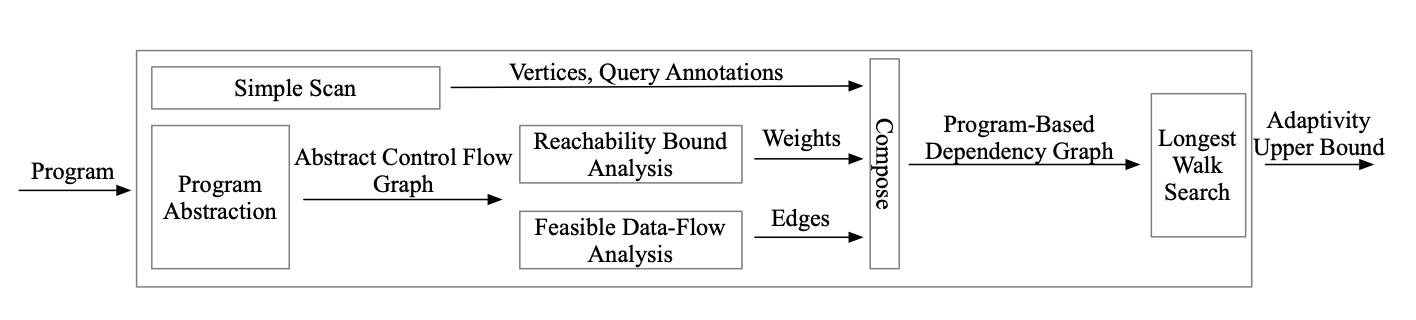
\includegraphics[width=\textwidth]{adapfun}
%   \caption{Seattle Mariners at Spring Training, 2010.}
%   \Description{Enjoying the baseball game from the third-base
%   seats. Ichiro Suzuki preparing to bat.}
%   \label{fig:teaser}
% \end{teaserfigure}

\received{20 February 2007}
\received[revised]{12 March 2009}
\received[accepted]{5 June 2009}

%%
%% This command processes the author and affiliation and title
%% information and builds the first part of the formatted document.
\maketitle

%%%%%%%%%%%%%%%%%%%%%%%%%%%%%%%%%%%%%%%%%%% Introduction and Overview %%%%%%%%%%%%%%%%%%%%%%%%%%%%%%%%%%%%%%%%%%% 
\section{Introduction}
\label{sec:intro}
\input{intro}
\section{Overview}
\label{sec:overview}
% Plan:
% \textbf{Two Examples + Algorithm Overview}
% \begin{itemize}
% \item {Multiple-Path While Loop}
% \\
% \textbf{The First Challenge/Problem from The Example, 
% and the Overview of the New Techniques Targeting This Problem}
% \item {Nested While Loop}
% \\
% \textbf{The Second Challenge/Problem from The Example,
% and the Overview of the New Techniques Targeting This Problem}
% \end{itemize}
In this section, we discuss two representative examples with
challenges of analyzing the symbolic
\emph{reachability-bound} on
every control location.
We also give the technique overview of our algorithm.
%
\subsection{Multiple-Path Loop}
\label{sec:overview-multiplepath}
    { \footnotesize
    \begin{figure}
    \centering
    %
    \begin{subfigure}{.27\textwidth}
        $
        \begin{array}{l}
          \kw{twoPathsWhile}(n, m) \triangleq \\
        \clabel{ \assign{i}{n} }^{0} ;
        \clabel{ \assign{j}{0} }^{1} ; \\
        L_2:    \ewhile ~ \clabel{i > 0}^{2} ~ \edo ~ \\
            \qquad \big(
              \eif(\clabel{j < m}^{3}, \\
              \qquad \ethen  \clabel{\assign{j}{j + 1}}^{4}; \\
              \qquad \qquad \clabel{\assign{i}{i - 1}}^{5},\\
              \qquad \eelse \clabel{\assign{j}{0}}^{6});
              \big)
            \end{array}
            $
\vspace{-0.2cm}
\caption{}
\end{subfigure}
\begin{subfigure}{.71\textwidth}
\begin{subfigure}{.67\textwidth}
\begin{centering}
\begin{tikzpicture}[scale=\textwidth/20cm,samples=200]
    \draw[] (-8, 10) circle (0pt) node{{ $0$}};
    \draw[] (-4, 10) circle (0pt) node{{ $1$}};
    \draw[] (0, 10) circle (0pt) node{{ $2$}};
    \draw[] (0, 7) circle (0pt) node{{$3$}};
    \draw[] (-3, 4) circle (0pt) node{{ $4$}};
    \draw[] (-8, 4) circle (0pt) node{{ $5$}};
    \draw[] (4, 4) circle (0pt) node{{ $6$}};
    % Counter Variables
    \draw[] (5, 10) circle (0pt) node {\textbf{$\lex$}};
    %
    % Control Flow Edges:
    \draw[ thick, -latex] (-7, 10)  -- node [above] {$i' \leq n$}(-4.5, 10);
    \draw[ thick, -latex] (-3, 10)  -- node [above] {$j' \leq 0$}(-0.5, 10);
    \draw[ thick, -latex] (0, 9.5)  -- node [left] {$i > 0$} (0, 7.5) ;
    \draw[ thick, -latex] (0.5, 7)  -- node [below] {$ j \geq m $}  (4, 4.5);
    \draw[ thick, -latex] (-7.5, 4.5)  to  [out=90,in=180]  node [left] {$i' \leq i - 1$ }(-0.5, 9.5);
    \draw[ thick, -latex] (4.5, 4)  to  [out=70,in=0]   node [right] {$j' \leq 0 $}(0.5, 9.5);
    \draw[ thick, -latex]  (-0.5, 7) -- node  {$j < m$}  (-3, 4.5) ;
    \draw[ thick, -latex]  (-3.5, 4) -- node [above] {$j' \leq j + 1$}  (-7, 4) ;
    \draw[ thick, -latex] (0.5, 10)  -- node [above] {$i \leq 0$}  (4.5, 10);
  \end{tikzpicture}
        \caption{}
\end{centering}
\end{subfigure}
{\small
\begin{subfigure}{.3\textwidth}
\begin{centering}
        $\tpath_0 = 0 \to 1 \to 2$ \\
        $\tpath_2 = 2 \to 3 \to 6 \to 2$ \\ 
        $\tpath_1 = 2 \to 3 \to 4 \to 5 \to 2$ \\
        $\tpath_3 = 2 \to \lex$
        \caption{}
\end{centering}
\end{subfigure}
}
{\small
\begin{subfigure}{.8\textwidth}
\begin{centering}
    $
    \tpath_0 ; 
    \rpchoose{2: \rprepeat(\rprepeat(\tpath_1); \tpath_2), 
    2: \rprepeat(\tpath_1)}; \tpath_3.
    $
\end{centering}
\end{subfigure}
}
\end{subfigure}
\vspace{-0.2cm}
\caption{
    (a) The two paths loop example,
    (b) the Abstract Transition Graph for $\kw{twoPathsWhile}(n, m)$,
    (c) the Simple Transition Paths of $\kw{twoPathsWhile}(n, m)$.}
    \vspace{-0.5cm}
        \label{fig:whileTwoCounters-overview}
    \end{figure}
    }



Figure~\ref{fig:whileTwoCounters-overview}(a) shows an example of a two paths loops
with different \emph{reachability-bounds} on the control locations in different paths.
This example is adopted from the example in~\cite{Sumit2010rechability}, which
is a skeleton code from the .Net base-class library.
\\
In this example, given $n \geq m$,
the precise \emph{reachability-bound}s for control locations $4$ and $5$ are both $m \times \lfloor\frac{n}{m}\rfloor$,
for location $2$ and $3$ are $(m + 1) \times \lfloor\frac{n}{m}\rfloor + 1$, 
and $1$ for locations $0, 1$ and $\lex$. 
\highlight{Notice here, though within the same loop $L_2$, the bounds for locations $4$ and $5$ on the first branch, and $6$ on the second branch are different.}
% \\
% In order to know that the locations in first branch ($4$ and $5$) are reached at most $m \times \lfloor\frac{n}{m}\rfloor$ times
% while $6$ in second branch $\lfloor\frac{n}{m}\rfloor$ times
%  during program execution,
% we need to know that the two if branches are interleaved and executed alternatively after each other
% during the iterations of the enclosed loop.
\\
However, the state-of-art \emph{reachability-bound} analysis~\cite{Sumit2010rechability}
gives the same \emph{reachability-bound}, $n + \lfloor\frac{n}{m}\rfloor$ for all the locations within the loop $L_2$, which is tight w.r.t. $L_2$'s iteration times but not for different locations inside $L_2$ without considering multiple paths.
Among works on program complexity, cost and loop bound analysis, \cite{GulwaniJK09} can also compute the tight bound on the loop iteration but not reachability-bound on each location path-sensitively.
Though we can use it as the \emph{reachability-bound} for location $1$ and $2$,
the \emph{reachability-bounds} for control locations $4, 5$ and $6$ are still unclear.
\paragraph{Path Reachability-bound}
To compute the bounds for locations on different paths of a loop, we compute the \emph{path reachability-bound},
which is the first key idea of this path-sensitive \emph{reachability-bound} analysis algorithm. This bound approximate the evaluation times of each loop free path instead of the entire multipath loop.
\\
% Our algorithm combines the idea of \emph{difference constraint} based program complexity analysis method from \cite{sinn2017complexity}
% and the control-flow refinement technique from~\cite{GulwaniJK09}.
For this example, we first
generate the abstract transition graph for the program using the difference constraints, such as Figure~\ref{fig:whileTwoCounters-overview}(b).
Then it transforms every the loop in $\kw{twoPathsWhile}$ using the control-flow refinement technique from~\cite{GulwaniJK09} and generates a refined program $\rprog$ as
\\
% 
% The refined program for program $\kw{twoPathsWhile}$ is
% \[
  $
  \tpath_0 ; 
  \rpchoose{2: \rprepeat_2(\rprepeat_1(\tpath_1); \tpath_2), 
  2: \rprepeat_1(\tpath_1)}; \tpath_3.
  $
% \]
\\
Each $\tpath_i$ in this refined program is a \emph{simple transition path} we computed in a pre-procedure, which is loop free and not interleave with the other $\tpath_j, j \neq i$ as in Figure~\ref{fig:whileTwoCounters-overview}(c).
% Every path will not interleave with the others. 
Then we compute the \emph{path reachability-bound} for every $\tpath_i$,
$\inoutB(\rprog, \tpath_i)$ during the execution of $\rprog$.
% which is a bound on the reachability time of $\tpath$ during the execution of $\rprog$.
The \emph{path reachability-bound}s for the four simple transition paths in this example are
$\inoutB(\rprog, \tpath_1) = \max\{m, m \times \lfloor\frac{n}{m}\rfloor\}$,
$\inoutB(\rprog, \tpath_2) = \lfloor\frac{n}{m}\rfloor$,
and $\inoutB(\rprog, \tpath_0) = \inoutB(\rprog, \tpath_3) = 1$.
% \\
% Then we use this bounds
% and another \emph{loop reachability-bound}
% to compute the final \emph{reachability-bound} for each location.
Since there isn't nested loop in this example, we simply sum up $\inoutB(\rprog, \tpath)$ over the $\tpath$ where a certain location shows up
and as the \emph{reachability-bound} of this location.
Then we get the precise \emph{reachability-bound} for every location in program $\kw{twoPathsWhile}$ as
$\psRB(0) = \psRB(1) = \psRB(\lex) = 1$,
$\psRB(4) = \psRB(5) = \max\{m, m \times \lfloor\frac{n}{m}\rfloor\}$,
$\psRB(3) = \psRB(2) = \max\{m, m \times \lfloor\frac{n}{m}\rfloor\} + \lfloor\frac{n}{m}\rfloor + 1 $,
and $\psRB(6) = \lfloor\frac{n}{m}\rfloor$.
%
\subsection{Nested Loops with Related Iterator}
\label{sec:overview-nestedwhile}
However, when there exists nested loop, computing the \emph{reachability-bound} for each location encounters another challenge.
The \emph{path reachability-bound} is precise for each path w.r.t. the innermost loop but not the outer nested loops.
Figure~\ref{fig:threeWhile-overview}(a) shows an example of the nested loops with related 
iterators.
This example is adopted from the example in~\cite{GulwaniJK09}, which is common in product code.
\\
In line 8, $i$ is reset by $w$ and $w$ is reset by $j$ at line 5. So the
while $L_6$ is only executed in the first iteration of while loop $L_1$ and $L_3$.
% \\
The while loop $L_3$ at line 3 is executed only in 
the first $m - N$ iterations of the 
$L_1$ because $j$ is reset by $i$ in line 2.
% \\
So the total iterations of all the three loops is
$n + m^2 - m \times N$,
and the precise \emph{reachability-bound} for location $7$ inside the $L_6$ is $N$,
for locations $4, 5$ and $8$ between the $L_3$ and $L_6$ are $(n-N) \times (m - N)$,
and $n - N$ for locations $2$ and $9$.
% \\
\highlight{Notice here the \emph{reachability-bounds} for the locations inside the loop $L_6$ is 
the same as its loop iteration bound, as well as our \emph{path reachability-bound}.
However, for the locations between $L_3$ and $L_6$,
the \emph{reachability-bounds} are the multiplication of the inner and outer loop iteration bounds.}
\\
To the best of our knowledge, the loop bound analysis method in \cite{GulwaniJK09} can only give a loose bound $n + (m \times n) + N$ for the entire loop complexity, and 
the DC-based algorithm in \cite{sinn2017complexity} is able to
compute a better but still loose bound, $n + m^2 - m \times N$ on total iteration times.
None of them can give the precise \emph{reachability-bound} for every location in these nested loops,
which is non-trivial to compute even though knowing the loop bound,
especially for the locations similar to $7$ in $\kw{threeNestedWhile}$.
\\
\highlight{
In order to precisely compute how many times the location $7$ is reached, we need to know
the numbers of iterations of the outside loop $L_3$ and $L_1$ such that,
during these iterations, the loop $L_6$ is ``entered''. 
We call this the \emph{loop reachability} of the location within loop $L_6$ w.r.t the loops $L_3$ and $L_1$.
Then by multiplying the loop iteration bound of the $L_6$ with its \emph{loop reachability} times w.r.t the  $L_3$ and $L_1$, we can compute the precise
\emph{reachability-bounds} for location $7$.
}
\\
\highlight{
This quantity isn't considered or computed in any of the previous works.
The \emph{Progress Invariant} method in \cite{GulwaniJK09} is only able to compute
the
bound on iteration numbers
of the inner loop $L_6$ in each iteration of $L_3$ and $L_1$, which are both $N$.
So they have to over-approximate the reachability-bound for locations inside $L_6$ with the
overall program complexity, i.e., $n + m^2 - m \times N$.
% \\
For the same reason, the DC-based algorithm in \cite{sinn2017complexity}
is only able to
compute the precise combined loop bound and the local bound of each loop
separately as well.
% We are still unable to know the precise \emph{reachability-bound} for the locations in the innermost loop.
}
\paragraph*{Loop reachability-bound.}
In this sense, this \emph{loop reachability-bound}, $\lpchB(L:\rprog, \tpath)$ is our second key idea.
For each transition path $\tpath$ w.r.t each of the loops $L:\rprog$ in which $\tpath$ is nested,
$\lpchB(L:\rprog, \tpath)$ 
\highlight{is a bound on the iterations for
the outside loop, $L:\rprog$ w.r.t. the innermost loop where $\tpath$ is enclosed,
such that during these iterations of $L:\rprog$, the innermost loop is ``entered''. 
This is distinguished from the traditional methods, which only estimate the bound on the inner loop's iteration number
in one iteration of the outside loop.}
\\
Similar to the $\kw{twoPathsWhile}$ example, we also generate its abstract transition graph as well in Figure~\ref{fig:threeWhile-overview}(a),
and compute its refined program,
$\rprog = \tpath_0; 1: \rprepeat(\tpath_1;$ 
$3: {\rprepeat(\tpath_2; 6 : {\rprepeat(\tpath_3)}; \tpath_4)}; \tpath_5);$ 
$\tpath_6$,
where the $\tpath_0, \ldots$ are shown in the middle part of Figure~\ref{fig:threeWhile-overview}(b).
We use $\rprog_1$ and $\rprog_3$ denote the body of the loop $L_1$ and $L_3$ respectively as in the bottom part of Figure~\ref{fig:threeWhile-overview}(b).
% to denote ${\rprepeat(\tpath_1; 3: {\rprepeat(\tpath_2; 6 : {\rprepeat(\tpath_3)}; \tpath_4)}; \tpath_5)}$
% and $\rprog_3 = {\rprepeat(\tpath_2; 6 : {\rprepeat(\tpath_3)}; \tpath_4)}$
In the first step, we still compute the \emph{path reachability-bound} for each $\tpath_i$ but only w.r.t. the closest loop it is nested.
Then differently from $\kw{twoPathsWhile}$,
we compute \emph{loop reachability-bound} for each $\tpath_i$ w.r.t. each of its nested loops.
For example, for $\tpath_3$ we compute
$\lpchB(1: \rprog_1, \tpath_3) = 1$ and
$\lpchB(3: \rprog_3, \tpath_3) = 1$.
Both are tight because loop $L_6$ will only be entered once among all iterations of $L_1$ and $L_3$, and in all the rest iterations, the body of loop $L_6$ isn't executed at all.
So $1$ as \emph{loop reachability-bound} of this path is tight w.r.t. both the loop $L_3$ and $L_1$.
% In the same way, we also compute $\lpchB(3: \rprog_3, \tpath_3) = 1$ precisely.
Then for each $\tpath_i$, the multiplication of its \emph{path reachability-bound} with all its \emph{loop reachability-bound}s is an accurate \emph{loop reachability-bound} for the locations on this path.
By summing up the reachability-bound of the path where each location shows up,
% as its \emph{reachability-bound} as before.
% and multiply this result by all its \emph{loop reachability-bound}s.
% In this way, 
we compute $N$ as the \emph{reachability-bound} of location $7$, which is tight.
    %
    \begin{figure}
    \centering
    %
    \vspace{-0.8cm}
    \begin{subfigure}{.45\textwidth}
        $
        \begin{array}{l}
            N < m < n\\
            \kw{threeNestedWhile}(n, m, N) \triangleq \\
            \clabel{ \assign{i}{0} }^{0} ; \\
                L_1: \ewhile ~ \clabel{i < n}^{1} ~ \edo ~ \\
                \quad (
                 \highlight{\clabel{\assign{j}{0}}^{2}} ;\\
                 L_3:  \quad \ewhile ~ \clabel{j < m}^{3} ~ \edo ~ \\
                \quad \quad ( \clabel{\assign{j}{j+1}}^{4};\\
                  \quad \quad \highlight{\clabel{\assign{w}{i}}^{5}};\\
                  L_6:  \quad \quad \ewhile ~ \clabel{w < N}^{6} ~ \edo ~ \\
                  \quad \quad \quad ( \clabel{\assign{w}{w + 1}}^{7} ); \\
                      \quad \quad \clabel{\assign{i}{w}}^{8}
                      ); \\
                      \quad \clabel{\assign{i}{i+1}}^{9})
            \end{array}
            $
            \vspace{-0.2cm}
            \caption{}
        \end{subfigure}
    \begin{subfigure}{.48\textwidth}
        \begin{centering}
            \begin{tikzpicture}[scale=\textwidth/20cm,samples=200]
                \draw[] (-5, 10) circle (0pt) node{{ $0$}};
                \draw[] (0, 10) circle (0pt) node{{ $1$}};
                \draw[] (6, 10) circle (0pt) node {{$\lex$}};
                \draw[] (0, 7) circle (0pt) node{{$2$}};
                \draw[] (0, 4) circle (0pt) node{{ $3$}};
                \draw[] (-5, 4) circle (0pt) node{{ $9$}};
                \draw[] (0, 1) circle (0pt) node{{ $4$}};
                \draw[] (4, 1) circle (0pt) node{{ $5$}};
                \draw[] (8, 1) circle (0pt) node{{ $6$}};
                \draw[] (13, 1) circle (0pt) node{{ $7$}};
                \draw[] (5, 6) circle (0pt) node{{ $8$}};
                % Counter Variables
                %
                % Control Flow Edges:
                \draw[ thick, -latex] (-4, 10)  -- node [above] {$i \leq 0$}(-0.5, 10);
                \draw[ thick, -latex] (0, 9.5)  -- node [left] {$i < k$} (0, 7.5) ;
                \draw[ thick, -latex] (0, 6.5)  -- node [right] {$j \leq m$} (0, 4.5) ;
                \draw[ thick, -latex] (0, 3.5)  -- node [left] {$j > 0$} (0, 1.5) ;
                \draw[ thick, -latex] (-0.5, 4)  -- node [above] {$j \leq 0$} (-4.5, 4) ;
                \draw[ thick, -latex] (-4.5, 4.5)  to  [out=90,in=180]  node [left] {$i \leq i + 1$ }(-0.5, 9.5);
                \draw[ thick, -latex] (0.5, 10)  -- node [above] {$i \leq 0$}  (5.5, 10);
                \draw[ thick, -latex] (0.5, 1)  -- node [above] {{\footnotesize $j \leq j - 1$}}  (3.5, 1);
                \draw[ thick, -latex] (4.5, 1)  -- node [above] {$w \leq i$}  (7.5, 1);
                \draw[ thick, -latex] (8.5, 1)  -- node [above] {{\footnotesize $w < N$}}  (12.5, 1);
                \draw[ thick, -latex] (8, 1.5)  to [out=90,in=0] node [left] {{$w \geq N$}}  (5.5, 6);
                \draw[ thick, -latex] (13, 1.5)  to  [out=120,in=60] node [above] {$w \leq w + 1$}  (8, 1.5);
                \draw[ thick, -latex] (5, 6.5)  to  [out=120,in=0]  node [right] {$i \leq i - 1$ }(0.5, 9.5);
                \end{tikzpicture}
%     \caption{}
%     \end{centering}
%     \end{subfigure}
% \begin{subfigure}{.2\textwidth}    
% \begin{centering}
    {\small
$
    \begin{array}{ll}
        \tpath_0 = (0 \to 1)
        &
        \tpath_4 = (6 \to 8 \to 3)
        \\        
        \tpath_1 = (1 \to 2 \to 3)
        &
        \tpath_5 = (3 \to 9 \to 1)
        \\
        \tpath_2 = (3 \to 4 \to 5 \to 6)
        &
        \tpath_6 = (1 \to \lex)
        \\
        \tpath_3 = (6 \to 7 \to 6)
    \end{array}
$
}
\vspace{-0.2cm}
\caption{}
\end{centering}
\end{subfigure}
% $
%     \begin{array}{l}
%         \rprog_1 = {\rprepeat(\tpath_1; 3: {\rprepeat(\tpath_2; 6 : {\rprepeat(\tpath_3)}; \tpath_4)}; \tpath_5)}
%         \\
%         \rprog_3 = {\rprepeat(\tpath_2; 6 : {\rprepeat(\tpath_3)}; \tpath_4)}
%     \end{array}
% $
$\rprog = \tpath_0; 1: \rprepeat(\tpath_1; 3: {\rprepeat(\tpath_2; 6 : {\rprepeat(\tpath_3)}; \tpath_4)}; \tpath_5);\tpath_6$
\vspace{-0.2cm}
\caption{
    (a) An example of three nested loops with related iterators,
    (b) the abstract transition graph, simple transition paths and loop body.}
    \vspace{-0.8cm}
        \label{fig:threeWhile-overview}
    \end{figure}

%%%%%%%%%%%%%%%%%%%%%%%%%%%%%%%%%%%%%%%%%%% Language %%%%%%%%%%%%%%%%%%%%%%%%%%%%%%%%%%%%%%%%%%%
\section{Labeled Query  While  language }
\label{sec:loop_language}
{\input{whilelanguage}}
%%%%%%%%%%%%%%%%%%%%%%%%%%%%%%%%%%%%%%%%%%% Adaptivity %%%%%%%%%%%%%%%%%%%%%%%%%%%%%%%%%%%%%%%%%%% 
\section{Definition of Adaptivity}
\label{sec:adaptivity}
\input{adapt}
%%%%%%%%%%%%%%%%%%%%%%%%%%%%%%%%%%%%%%%%%%% Adaptfun %%%%%%%%%%%%%%%%%%%%%%%%%%%%%%%%%%%%%%%%%%% 
\section{The Adaptivity Analysis Algorithm - {\THESYSTEM}}
\label{sec:algorithm}
{\input{adaptfun}}
%%%%%%%%%%%%%%%%%%%%%%%%%%%%%%%%%%%%%%%%%%% Evaluation %%%%%%%%%%%%%%%%%%%%%%%%%%%%%%%%%%%%%%%%%%% 
\section{Examples}
\label{sec:examples}
\subsection{Two Paths While Loop Example}
\begin{example}[While with Two Paths]
  \label{ex:twoPathsWhile}
  %
  { \small
  \begin{figure}
  \centering
  \begin{subfigure}{.4\textwidth}
    \begin{centering}
    {\small
    $
    \begin{array}{l}
      \kw{twoPathsWhile}(n, m) \triangleq \\
    \clabel{ \assign{i}{n} }^{0} ; \\
    \clabel{ \assign{j}{0} }^{1} ; \\
        \ewhile ~ \clabel{i > 0}^{2} ~ \edo ~ \\
        \qquad \Big(
          \eif(\clabel{j < m}^{3}, \\
          \qquad \qquad \clabel{\assign{j}{j + 1}}^{4}; 
          \clabel{\assign{i}{i - 1}}^{5},\\
          \qquad \qquad \clabel{\assign{j}{0}}^{6});
          \Big)
        \end{array}
        $
    }
    \caption{}
    \end{centering}
    \end{subfigure}
  \begin{subfigure}{.5\textwidth}
    \begin{centering}
  %   \todo{abstract-cfg for two round}
  \begin{tikzpicture}[scale=\textwidth/20cm,samples=200]
  \draw[] (-8, 10) circle (0pt) node{{ $0$}};
  \draw[] (-4, 10) circle (0pt) node{{ $1$}};
  \draw[] (0, 10) circle (0pt) node{{ $2$}};
  \draw[] (0, 7) circle (0pt) node{{$3$}};
  \draw[] (-3, 4) circle (0pt) node{{ $4$}};
  \draw[] (-8, 4) circle (0pt) node{{ $5$}};
  \draw[] (4, 4) circle (0pt) node{{ $6$}};
  % Counter Variables
  \draw[] (6, 10) circle (0pt) node {\textbf{$\lex$}};
  % \draw[] (6, 4) circle (0pt) node {{ $ex$}};
  %
  % Control Flow Edges:
  \draw[ thick, -latex] (-7, 10)  -- node [above] {$i' \leq n$}(-4.5, 10);
  \draw[ thick, -latex] (-3, 10)  -- node [above] {$j' \leq 0$}(-0.5, 10);
  \draw[ thick, -latex] (0, 9.5)  -- node [left] {$i > 0$} (0, 7.5) ;
  \draw[ thick, -latex] (0.5, 7)  -- node [below] {$ j \geq m $}  (4, 4.5);
  \draw[ thick, -latex] (-7.5, 4.5)  to  [out=90,in=180]  node [left] {$i' \leq i - 1$ }(-0.5, 9.5);
  \draw[ thick, -latex] (4.5, 4)  to  [out=70,in=0]   node [right] {$j' \leq 0 $}(0.5, 9.5);
  \draw[ thick, -latex]  (-0.5, 7) -- node  {$j < m$}  (-3, 4.5) ;
  \draw[ thick, -latex]  (-3.5, 4) -- node [above] {$j' \leq j + 1$}  (-7, 4) ;
  \draw[ thick, -latex] (0.5, 10)  -- node [above] {$i \leq 0$}  (5.5, 10);
  % \draw[ thick, -latex] (6, 6.5)  -- node [right] {$\top$} (6, 4.5) ;
  \end{tikzpicture}
  \caption{}
    \end{centering}
    \end{subfigure}
  \caption{
  (a) The Two Paths While Loop Example
    (b) The Abstract Execution Control Flow Graph}
      \label{fig:twoPathsWhile}
  \end{figure}
  }
\end{example}

\begin{enumerate}
  \item  \textbf{The Abstract Execution Control Flow Graph} is generated in Figure~\ref{fig:twoPathsWhile}(b).

  \item \textbf{Program Rephrase and Refinement}. 
  \\
  The loop free simple transition paths are computed as follows,
  \[
    \begin{array}{ll}
\tpath_0 = (0 \to 1), (1 \to 2)
&
\tpath_2 = (2 \to 3), (3 \to 6), (6 \to 2)
\\
\tpath_1 = (2 \to 3), (3 \to 4), (4 \to 5), (5 \to 2)
&
\tpath_3 = (2 \to \lex)
\end{array}
\]
\textbf{Refined Program}:
\[
  \tpath_0 ; \rpchoose{2: \rprepeat_2(\rprepeat_1(\tpath_1); \tpath_2) , 
  2: \rprepeat_1(\tpath_1) }; \tpath_3
  \]
  \item \textbf{Ranks}:
  The ranking bounds for every simple transition path:
  \\
  $\absclr(\tpath_0) = 1$ 
  $\absclr(\tpath_1) = n $ \quad
  $\absclr(\tpath_2) = n $ \quad
  $\absclr(\tpath_3) = 1$
  % \\
  % $\bot$ means the algorithm fails in inferring the ranking bound.
    \item \textbf{Outside-In Algorithm} :The \emph{OutIn} bound for the $\rprog$ and every nested repeat patterns.
  \[
    \begin{array}{l}
        \outinB(\tpath_0) = 1
        \\
        \outinB(2: \rprepeat_1(\tpath_1)) = m 
        \\
        \outinB(2: \rprepeat_2(\rprepeat_1(\tpath_1); \tpath_2)) = \lfloor\frac{n}{m}\rfloor
        \\
        \outinB(\rpchoose{\rprepeat_2(\rprepeat_1(\tpath_1); \tpath_2), \rprepeat_1(\tpath_1) })
        = \max\{m, (m  + 1)\times \lfloor\frac{n}{m}\rfloor\}
\end{array}
\]
\item \textbf{Inside-Out Algorithm}
\begin{itemize}
  \item \textbf{Repeat Chain Set}
  \\
  $\rpchset(2, \tpath_1) = \{\rprepeat_1(\tpath_1), \rprepeat_2(\rprepeat_1(\tpath_1); \tpath_2) \to \rprepeat_1(\tpath_1)\}$ \\
  $\rpchset(2, \tpath_2) = \{\rprepeat_2(\rprepeat_1(\tpath_1); \tpath_2) \to \rprepeat_1(\tpath_1)\}$ \\
  $\rpchset(\_, \_) = \emptyset$ 
  % \\
  \item \textbf{Repeat Chain Bound} for every simple transition path $\tpath$ through its \emph{Repeat Chain}s
  \\
  $\rpchB(2, \tpath_1) = \max\{m, m \times \lfloor\frac{n}{m}\rfloor\}$ \\
  $\rpchB(2, \tpath_2) = \lfloor\frac{n}{m}\rfloor$ 
  %
  \item \textbf{Loop Chain}
  \\
  $\lpch(\tpath_0) = \tpath_0$ \qquad
  $\lpch(\tpath_1) = 2\to \tpath_1$ \\
  $\lpch(\tpath_3) = \tpath_3$ \qquad
  $\lpch(\tpath_2) = 2\to \tpath_2$ 
  \item \textbf{{Relative Loop Bound}} for every simple transition path $\tpath$ through its \emph{Loop Chain}
  \\
  $\rpchB(2, \tpath_1) = \max\{m, m \times \lfloor\frac{n}{m}\rfloor\}$ \quad
  $\rpchB(2, \tpath_2) = \lfloor\frac{n}{m}\rfloor$  \\
  $\rpchB(\bot, \tpath_0) = 1$ \quad
  $\rpchB(\bot, \tpath_3) = 1$ 
  \item \textbf{Path-Sensitive Reachability-Bound} for every simple transition path $\tpath$
  \\
  $\inoutB(\tpath_1) = n$ \quad
  $\inoutB(\tpath_2) = \lfloor\frac{n}{m}\rfloor$ \quad
  $\inoutB(\tpath_0) = 1$ \quad
  $\inoutB(\tpath_3) = 1$ 
\end{itemize}
\item \textbf{Path Sensitive Reachability-Bound} on every program control location
\\
$\psRB(\{0, 1, \lex\}) = 1$ \qquad
$\psRB(\{6 \}) = \lfloor\frac{n}{m}\rfloor$ \\
$\psRB(\{4, 5 \}) = \max\{m, m \times \lfloor\frac{n}{m}\rfloor\}$ \quad
$\psRB(\{3, 2 \}) = \max\{m, m \times \lfloor\frac{n}{m}\rfloor\} + \lfloor\frac{n}{m}\rfloor + 1 $ \\
\end{enumerate}
\subsection{Three Nested While Loop with Related Iterator Example}
\begin{example}[Nested Loop with Related Iterators]
  \label{ex:threeNestedWhile}
  %
  %
  { \small
\begin{figure}
\centering
\begin{subfigure}{.4\textwidth}
  \begin{centering}
  {\footnotesize
  $
  \begin{array}{l}
      \kw{relatedNestedWhile}(n, m, N) \triangleq \\
      \clabel{ \assign{i}{0} }^{0} ; \\
          \ewhile ~ \clabel{i < n}^{1} ~ \edo ~ \\
          \qquad \Big(
           \clabel{\assign{j}{m}}^{2} ;\\
           \qquad \ewhile ~ \clabel{j > 0}^{3} ~ \edo ~ \\
           \qquad \qquad \Big(
            \clabel{\assign{j}{j-1}}^{4};
            \clabel{\assign{w}{i}}^{5};\\
            \qquad \qquad \ewhile ~ \clabel{w < N}^{6} ~ \edo ~
            \Big(
              \clabel{\assign{w}{w + 1}}^{7}
                \Big); \\
                \qquad \qquad \clabel{\assign{i}{w}}^{8}
                \Big); \\
                \qquad \clabel{\assign{i}{i+1}}^{9}
            \Big)
      \end{array}
  $
  }
  \caption{}
  \end{centering}
  \end{subfigure}
\begin{subfigure}{.5\textwidth}
  \begin{centering}
%   \todo{abstract-cfg for two round}
\begin{tikzpicture}[scale=\textwidth/20cm,samples=200]
\draw[] (-7, 10) circle (0pt) node{{ $0$}};
\draw[] (0, 10) circle (0pt) node{{ $1$}};
\draw[] (6, 10) circle (0pt) node {{$\lex$}};
\draw[] (0, 7) circle (0pt) node{{$2$}};
\draw[] (0, 4) circle (0pt) node{{ $3$}};
\draw[] (-7, 4) circle (0pt) node{{ $9$}};
\draw[] (0, 1) circle (0pt) node{{ $4$}};
\draw[] (3, 1) circle (0pt) node{{ $5$}};
\draw[] (6, 1) circle (0pt) node{{ $6$}};
\draw[] (9, 1) circle (0pt) node{{ $7$}};
\draw[] (5, 6) circle (0pt) node{{ $8$}};
% Counter Variables
%
% Control Flow Edges:
\draw[ thick, -latex] (-6, 10)  -- node [above] {$i' \leq 0$}(-0.5, 10);
\draw[ thick, -latex] (0, 9.5)  -- node [left] {$i < n$} (0, 7.5) ;
\draw[ thick, -latex] (0, 6.5)  -- node [left] {$j' \leq m$} (0, 4.5) ;
\draw[ thick, -latex] (0, 3.5)  -- node [left] {$j > 0$} (0, 1.5) ;
\draw[ thick, -latex] (-0.5, 4)  -- node [below] {$j \leq 0$} (-6.5, 4) ;
\draw[ thick, -latex] (-6.5, 4.5)  to  [out=90,in=180]  node [left] {$i' \leq i + 1$ }(-0.5, 9.5);
\draw[ thick, -latex] (0.5, 10)  -- node [above] {$i \geq n$}  (5, 10);
\draw[ thick, -latex] (0.5, 1)  -- node [below] {$j' \leq j - 1$}  (2.5, 1);
\draw[ thick, -latex] (3.5, 1)  -- node [above] {$w' \leq i$}  (5.5, 1);
\draw[ thick, -latex] (6.5, 1)  -- node [below] {$w < N$}  (8.5, 1);
\draw[ thick, -latex] (6, 1.5)  to [out=90,in=-60] node [right] {$w \geq N$}  (5, 5.5);
\draw[ thick, -latex] (9, 1.5)  to  [out=120,in=30] node [right] {$w' \leq w + 1$}  (6, 1.5);
\draw[ thick, -latex] (5, 5.5)  to  node [above] {$i' \leq k$ }(0.5, 4);
\end{tikzpicture}
\caption{}
  \end{centering}
  \end{subfigure}
\caption{
(a) The Example of Nested Loop with Related Iterators
  (b) The Abstract Execution Control Flow Graph}
    \label{fig:threeNestedWhile}
\end{figure}
}
\end{example}

\begin{enumerate}
  \item  \textbf{The Constraint Program (Abstract Control Flow Graph)} is generated in Figure~\ref{fig:threeNestedWhile}(b).

  \item \textbf{Program Refinement}
  \\
  The loop free simple transition paths are computed as follows,
  \[
      \begin{array}{llll}
          \tpath_0 = (0 \to 1)
          &
          \tpath_1 = (1 \to 2), (2 \to 3)
          &           
          \tpath_2 = (3 \to 4), (4 \to 5), (5 \to 6)
          &
          \tpath_3 = (6 \to 7), (7 \to 6)
          \\
          \tpath_6 = (1 \to \lex)
          &
          \tpath_4 = (6 \to 8), (8 \to 3)
          &
          \tpath_5 = (3 \to 9), (9 \to 1)
      \end{array}
      \]
  \textbf{Refined Program}:
  \[
  \rprog = \tpath_0 ; 1: \rprepeat(\tpath_1; 3: \rprepeat(\tpath_2; 6 : \rprepeat(\tpath_3); \tpath_4); \tpath_5); \tpath_6
  \]
  \item \textbf{Outside-In Algorithm} :The \emph{OutIn} bound for the $\rprog$ and every nested repeat patterns.
  \\
$\outinB(\tpath_0) = 1$
\quad
$\outinB(\tpath_6) = 1$
\quad
$\outinB(6 : \rprepeat(\tpath_3)) = N $
\\
$\outinB(3: \rprepeat(\tpath_2; 6 : \rprepeat(\tpath_3); \tpath_4)) = m $
\\
$\outinB(1: \rprepeat(\tpath_1; 3: \rprepeat(\tpath_2; 6 : \rprepeat(\tpath_3); \tpath_4); \tpath_5)) = n - N $
\item \textbf{Inside-Out Algorithm}
\begin{itemize}
  \item \textbf{Repeat Chain Set}
  \\
  $\rpchset(1, \tpath_1) = \{1: \rprepeat(\tpath_1; 3: \rprepeat(\tpath_2; 6 : \rprepeat(\tpath_3); \tpath_4); \tpath_5)\}$
  \\
  $\rpchset(1, \tpath_5) = \{1: \rprepeat(\tpath_1; 3: \rprepeat(\tpath_2; 6 : \rprepeat(\tpath_3); \tpath_4); \tpath_5)\}$
  \\
  $\rpchset(3, \tpath_2) = \{3: \rprepeat(\tpath_2; 6 : \rprepeat(\tpath_3); \tpath_4)\}$
  \\
  $\rpchset(3, \tpath_4) = \{3: \rprepeat(\tpath_2; 6 : \rprepeat(\tpath_3); \tpath_4)\}$
  \\
  $\rpchset(6, \tpath_3) = \{6: \rprepeat(\tpath_3)\}$
  \\
  $\rpchset(_, \_) = \emptyset$ 
  % \\
  \item \textbf{Repeat Chain Bound} for every simple transition path $\tpath$ through its \emph{Repeat Chain}s
  \\
  $\rpchB(1, \tpath_1) = n - N$ \quad
  $\rpchB(1, \tpath_5) = n - N$ \quad
  $\rpchB(3, \tpath_2) = m$ \\
  $\rpchB(3, \tpath_4) = m$ \quad
  $\rpchB(6, \tpath_3) = N$ \quad \quad 
  $\rpchB(_, \_) = \bot $ 
  %
  \item \textbf{Loop Chain}
  \\
  $\lpch(\tpath_1) = 1\to \tpath_1$ \quad
  $\lpch(\tpath_2) = 1 \to 3 \to \tpath_2$ \\
  $\lpch(\tpath_5) = 1\to \tpath_5$ \quad
  $\lpch(\tpath_4) = 1 \to 3 \to \tpath_4$ \\
  \highlight
  {$\lpch(\tpath_3) = 1 \to 3 \to 5 \to \tpath_3$ }\\
  $\lpch(\tpath_0) = \tpath_0$ \quad
  $\lpch(\tpath_6) = \tpath_6$ 
  \item \textbf{{Relative Loop Bound}} for every simple transition path $\tpath$ through its \emph{Loop Chain}
  \\
  $\rpchB(1, \tpath_1) = n - N$ \\
  $\rpchB(1, \tpath_5) = n - N$ \\
  $\rpchB(1, \tpath_2) = n$; \quad $\rpchB(3, \tpath_2) = m$; \\
  $\rpchB(1, \tpath_4) = n$; \quad $\rpchB(3, \tpath_4) = m$ \\
  \highlight{$\rpchB(1, \tpath_3) = 1$; \quad $\rpchB(3, \tpath_3) = 1$; \quad $\rpchB(5, \tpath_3) = N$} \\
  $\rpchB(_, \_) = \bot $ 
  \item \textbf{Path-Sensitive Reachability-Bound} for every simple transition path $\tpath$
  \\
  $\inoutB(\tpath_1) = n - N$ \quad
  $\inoutB(\tpath_2) = n \times m$ \quad
  $\inoutB(\tpath_0) = 1$ 
  \\
  $\inoutB(\tpath_5) = n - N$ \quad
  $\inoutB(\tpath_4) = n \times m$ \quad
  $\inoutB(\tpath_6) = 1$ 
  \\
  $\inoutB(\tpath_3) = N$ \quad
\end{itemize}
\item \textbf{Path Sensitive Reachability-Bound} on every program control location
\\
$\psRB(\{0, \lex\}) = 1$ \quad
$\psRB(\{1\}) = n - N + 1$ \quad
$\psRB(\{2, 9\}) = n - N$ \quad
$\psRB(\{3\}) = n - N + n \times m$ \quad
$\psRB(\{4, 5, 8\}) = n \times m$ \quad
$\psRB(\{7\}) = N$ \quad
$\psRB(\{6\}) = N + n \times m$ 
\end{enumerate}
\subsection{Simplified Nested Loop with Related Iterator Example}
\begin{example}[Nested Loop with Related Iterator]
  \label{ex:relatedNestedWhileSim}
  %
  %
  { \small
\begin{figure}
\centering
\begin{subfigure}{.4\textwidth}
  \begin{centering}
  {\small
  $
  \begin{array}{l}
      \kw{relatedNestedWhileSim}(n, N) \triangleq \\
      \clabel{ \assign{i}{n} }^{0} ; \\
          \ewhile ~ \clabel{i > 0}^{1} ~ \edo ~ \\
          \qquad \Big(
            \clabel{\assign{k}{i - N}}^{2};\\
            \qquad \ewhile ~ \clabel{k > 0}^{3} ~ \edo ~
            \Big(
              \clabel{\assign{k}{k - 1}}^{4}
                \Big); \\
                \qquad \clabel{\assign{i}{k + N}}^{5};
                \clabel{\assign{i}{i-1}}^{6}
            \Big)
      \end{array}
  $
  }
  \caption{}
  \end{centering}
  \end{subfigure}
\begin{subfigure}{.5\textwidth}
  \begin{centering}
%   \todo{abstract-cfg for two round}
\begin{tikzpicture}[scale=\textwidth/20cm,samples=200]
\draw[] (-7, 10) circle (0pt) node{{ $0$}};
\draw[] (0, 10) circle (0pt) node{{ $1$}};
\draw[] (6, 10) circle (0pt) node {{$\lex$}};
\draw[] (0, 7) circle (0pt) node{{$2$}};
\draw[] (0, 4) circle (0pt) node{{ $3$}};
\draw[] (-7, 4) circle (0pt) node{{ $6$}};
\draw[] (-3, 4) circle (0pt) node{{ $5$}};
\draw[] (4, 4) circle (0pt) node{{ $4$}};
% Counter Variables
%
% Control Flow Edges:
\draw[ thick, -latex] (-6, 10)  -- node [above] {$i' \leq n$}(-0.5, 10);
\draw[ thick, -latex] (0, 9.5)  -- node [left] {$i > 0$} (0, 7.5) ;
\draw[ thick, -latex] (0, 6.5)  -- node [left] {$k' \leq i - N$} (0, 4.5) ;
\draw[ thick, -latex] (-0.5, 4)  -- node [below] {$k \leq 0$} (-2.5, 4) ;
\draw[ thick, -latex] (-3.5, 4)  -- node [below] {$i' \leq k + N$} (-6.5, 4) ;
\draw[ thick, -latex] (-6.5, 4.5)  to  [out=90,in=180]  node [left] {$i' \leq i - 1$ }(-0.5, 9.5);
\draw[ thick, -latex] (0.5, 10)  -- node [above] {$i \leq 0 $}  (5, 10);
\draw[ thick, -latex] (4, 4.5)  to  [out=120,in=30] node [above] {$k' \leq k - 1$}  (0.5, 4.5);
\draw[ thick, -latex] (0.5, 4)  -- node [below] {$k > 0$}  (3.5, 4);
\end{tikzpicture}
\caption{}
  \end{centering}
  \end{subfigure}
\caption{
(a) The Simplified Example of Nested Loop with Related Iterator
  (b) The Abstract Execution Control Flow Graph}
    \label{fig:relatedNestedWhileSim}
\end{figure}
}
\end{example}

\begin{enumerate}
  \item  \textbf{Abstract Control Flow Graph} is generated in Figure~\ref{fig:relatedNestedWhileSim}(b).

  \item \textbf{Program Refinement}
  \\
  The loop free simple transition paths:
  \[
      % \begin{array}{lllll}
          \tpath_0 = (0 \to 1)
          \quad
          \tpath_1 = (1 \to 2 \to 3)
          \quad           
          \tpath_2 = (3 \to 4 \to 3)
          \quad
          \tpath_3 = (3 \to 5 \to 6 \to 1)
          \quad
          \tpath_4 = (1 \to \lex)
      % \end{array}
      \]
  \textbf{Refined Program}:
  \[
  \rprog = \tpath_0 ; 1: \rprepeat(\tpath_1; 3: \rprepeat(\tpath_2); \tpath_3); \tpath_4
  \]
\item {Path Local Reachability Bound}:
\\
$\outinB(None, \tpath_0) = 1$ \quad
$\outinB(1: \rprog_1, \tpath_1) = N$ \quad
$\outinB(1: \rprog_1, \tpath_3) = N$ \quad
$\outinB(3: \rprog_3, \tpath_2) = n - N$ \\
$\outinB(None, \tpath_4) = 1$
%
\\
Loop Bounds:
\\
$BD(\tpath_0) = 1$
\quad
$BD(\tpath_4) = 1$
\quad
$BD(\rprepeat(\tpath_2)) = n - N $
\quad
$BD(\rprepeat(\tpath_1; 3: \rprepeat(\tpath_2); \tpath_3)) = N $
%
\item Loop Reachability Bound:
\\
\highlight{
$\lpchB(1: \rprog_1, \tpath_0) = 0$ \quad
$\lpchB(1: \rprog_1, \tpath_1) = N$ \quad
$\lpchB(1: \rprog_1, \tpath_3) = N$ \quad \\
$\lpchB(1: \rprog_1, \tpath_2) = 1$ \quad
$\lpchB(1: \rprog_1, \tpath_4) = 0$ \quad
$\lpchB(1: \rprog_3, \tpath_0) = 0$ \quad\\
% $\lpchB(1: \rprog_1, \tpath_1) = N$ \quad
% $\lpchB(1: \rprog_1, \tpath_3) = N$ \quad
$\lpchB(1: \rprog_3, \tpath_2) = n - N$ \quad
$\lpchB(1: \rprog_3, \tpath_4) = 0$ \quad
$\lpchB(3: \rprog_3, \tpath_4) = m$ 
}
%
%
\item Path Global Reachability Bound:
\\
$\inoutB(\rprog, \tpath_0) = 1$ \quad
$\inoutB(\rprog, \tpath_1) = N$ \quad
$\inoutB(\rprog, \tpath_2) = 1 \times (n - N)$ \quad
$\inoutB(\rprog, \tpath_3) = N$ \quad
$\inoutB(\rprog, \tpath_4) = 1$
%
\item The Reachability Bound:
\\
$\psRB(0) = \psRB(\lex) = 1$ \quad
$\psRB(1) = N + 1$ \quad
$\psRB(4) = n - N$ \quad \\
$\psRB(2) = \psRB(5) =  \psRB(6) = N$ \quad
\highlight{$\psRB(\{3\}) = N + 1 + n - N = n + 1$}
\end{enumerate}
\subsection{Nested Loop with Iterator Reset Chain Example}
\begin{example}[Nested Loop with Variable Reset Chain]
  \label{ex:nestedWhileResetChain}
  %
  %
  { \small
\begin{figure}
\centering
\begin{subfigure}{.4\textwidth}
  \begin{centering}
  {\small
  $
  \begin{array}{l}
      \kw{nestedWhileResetChain}(n) \triangleq \\
      \clabel{ \assign{i}{n} }^{0} ; \\
      \clabel{ \assign{r}{n} }^{1} ; \\
          \ewhile ~ \clabel{i > 0}^{2} ~ \edo ~ \\
          \qquad \Big( \clabel{\assign{r}{r + 1}}^{3};\\
            \qquad  \clabel{\assign{k}{r}}^{4};\\
            \qquad \ewhile ~ \clabel{k > 0}^{5} ~ \edo ~
            \Big( \clabel{\assign{k}{k - 1}}^{6}   \Big); \\
                \qquad \clabel{\assign{r}{k}}^{7};
                \clabel{\assign{i}{i-1}}^{8}
            \Big)
      \end{array}
  $
  }
  \caption{}
  \end{centering}
  \end{subfigure}
\begin{subfigure}{.5\textwidth}
  \begin{centering}
\begin{tikzpicture}[scale=\textwidth/20cm,samples=200]
\draw[] (-10, 10) circle (0pt) node{{ $0$}};
\draw[] (-5, 10) circle (0pt) node{{ $1$}};
\draw[] (0, 10) circle (0pt) node{{ $2$}};
\draw[] (4, 10) circle (0pt) node {{$\lex$}};
%
\draw[] (0, 7) circle (0pt) node{{$3$}};
\draw[] (0, 3.5) circle (0pt) node{{ $4$}};
\draw[] (0, 0) circle (0pt) node{{ $5$}};
\draw[] (4, 0) circle (0pt) node{{ $6$}};
%
\draw[] (-3, 0) circle (0pt) node{{ $7$}};
\draw[] (-7, 0) circle (0pt) node{{ $8$}};
% Counter Variables
%
% Control Flow Edges:
\draw[ thick, -latex] (-9, 10)  -- node [above] {$i' \leq n$}(-5.5, 10);
\draw[ thick, -latex] (-4, 10)  -- node [above] {$r' \leq n$}(-0.5, 10);
\draw[ thick, -latex] (0.5, 10)  -- node [above] {$i \leq 0 $}  (3, 10);
\draw[ thick, -latex] (0, 9.5)  -- node [left] {$i > 0$} (0, 7.5) ;
\draw[ thick, -latex] (0, 6.5)  -- node [left] {$r' \leq r + 1$} (0, 4) ;
\draw[ thick, -latex] (0, 3)  -- node [left] {$k' \leq r$} (0, 0.5) ;
% While Guard True, Loop Body
\draw[ thick, -latex] (0.5, 0)  -- node [below] {$k > 0$}  (3.5, 0);
\draw[ thick, -latex] (4, 0.5)  to  [out=120,in=30] node [right] {$k' \leq k - 1$}  (0.5, 0.5);
% While Guard IS FALSE, RETURN BACK TO THE PREVIOUS CONTROL POINT
\draw[ thick, -latex] (-0.5, 0)  -- node [below] {$k \leq 0$} (-2.5, 0) ;
\draw[ thick, -latex] (-3.5, 0)  -- node [below] {$r' \leq k$} (-6.5, 0) ;
\draw[ thick, -latex] (-6.5, 0.5)  to  [out=90,in=180]  node [left] {$i' \leq i - 1$ }(-0.5, 9.5);
\end{tikzpicture}
\caption{}
  \end{centering}
  \end{subfigure}
\caption{
(a) The Simplified Example of Nested Loop with Related Iterator
  (b) The Abstract Execution Control Flow Graph}
    \label{fig:nestedWhileResetChain}
\end{figure}
}
\end{example}

\begin{enumerate}
  \item  \textbf{Abstract Control Flow Graph} is generated in Figure~\ref{fig:nestedWhileResetChain}(b).

  \item \textbf{Program Refinement}
  \\
  The loop free simple transition paths:
  \[
      % \begin{array}{lllll}
          \tpath_0 = (0 \to 1 \to 2)
          \quad
          \tpath_1 = (2 \to 3 \to 4 \to 5)
          \quad           
          \tpath_2 = (5 \to 6 \to 5)
          \quad
          \tpath_3 = (5 \to 7 \to 8 \to 2)
          \quad
          \tpath_4 = (2 \to \lex)
      % \end{array}
      \]
  \textbf{Refined Program}:
  \[
  \rprog = \tpath_0 ; 2: \rprepeat(\tpath_1; 5: \rprepeat(\tpath_2); \tpath_3); \tpath_4
  \]
\item {Path Local Reachability Bound}:
\\
$\outinB(None, \tpath_0) = 1$ \quad
$\outinB(2: \rprog_1, \tpath_1) = n$ \quad
$\outinB(2: \rprog_1, \tpath_3) = n$ \quad
$\outinB(5: \rprog_5, \tpath_2) = 2n$ \\
$\outinB(None, \tpath_4) = 1$
%
\\
Loop Bounds:
\\
$BD(\tpath_0) = 1$
\quad
$BD(\tpath_4) = 1$
\quad
$BD(\rprepeat(\tpath_2)) = n - N $
\quad
$BD(\rprepeat(\tpath_1; 5: \rprepeat(\tpath_2); \tpath_3)) = N $
%
\item Loop Reachability Bound:
\\
\highlight{
$\lpchB(2: \rprog_1, \tpath_0) = 0$ \quad
$\lpchB(2: \rprog_1, \tpath_1) = n$ \quad
$\lpchB(2: \rprog_1, \tpath_3) = n$ \quad \\
$\lpchB(2: \rprog_1, \tpath_2) = \frac{n + 1}{n}$ \quad
$\lpchB(2: \rprog_1, \tpath_4) = 0$ \quad
$\lpchB(2: \rprog_3, \tpath_0) = 0$ \quad\\
$\lpchB(5: \rprog_3, \tpath_2) = n + 1$
}
%
%
\item Path Global Reachability Bound:
\\
$\inoutB(\rprog, \tpath_0) = 1$ \quad
$\inoutB(\rprog, \tpath_1) = n$ \quad
$\inoutB(\rprog, \tpath_2) = \frac{(n + 1)^2}{n}$ \quad
$\inoutB(\rprog, \tpath_3) = n$ \quad
$\inoutB(\rprog, \tpath_4) = 1$
%
\item The Reachability Bound:
\\
$\psRB(0) = \psRB(1) = \psRB(\lex) = 1$ \quad
$\psRB(2) = n + 1$ \quad
$\psRB(3) = \psRB(4) =\psRB(7) = \psRB(8) = n$ \quad \\
$\psRB(6) = \frac{(n + 1)^2}{n} $ \quad
\highlight{$\psRB(\{5\}) = n + \frac{(n + 1)^2}{n} + 1$}
\end{enumerate}
\subsection{Two Paths Loop with Nested Loop in One Path}
\begin{example}
  [Example with Two Paths Iterating Alternatively and Nested Loop in One Path]
  \label{ex:nestedWhileOdd}
  { \small
  \begin{figure}
  \centering
  \begin{subfigure}{.4\textwidth}
    \begin{centering}
    {\small
    $
    \begin{array}{l}
      \kw{nestedWhileOdd}(k) \triangleq \\
      \clabel{ \assign{i}{k} }^{0} ; \\
          \ewhile ~ \clabel{i > 0}^{1} ~ \edo ~ \\
          \qquad \Big(
            \eif(\clabel{i \% 2 = 0 }^{2},\\
            \qquad \clabel{\assign{i}{i - 1}}^{3};
            \clabel{\assign{j}{k}}^{4}; \\
            \qquad \ewhile ~ \clabel{j > 0}^{5} ~ \edo ~
            \Big( \clabel{\assign{j}{j - 1}}^{6} \Big),\\
            \qquad \clabel{\assign{i}{i - 3}}^{7});
            \Big)
      \end{array}
    $
    }
    \caption{}
    \end{centering}
    \end{subfigure}
  \begin{subfigure}{.5\textwidth}
    \begin{centering}
  \begin{tikzpicture}[scale=\textwidth/20cm,samples=200]
  \draw[] (-7, 10) circle (0pt) node{{ $0$}};
  \draw[] (0, 10) circle (0pt) node{{ $1$}};
  \draw[] (0, 7) circle (0pt) node{\textbf{$2$}};
  \draw[] (0, 4) circle (0pt) node{{ $3$}};
  \draw[] (-4, 4) circle (0pt) node{{ $4$}};
  \draw[] (-8, 4) circle (0pt) node{{ $5$}};
  \draw[] (-8, 1) circle (0pt) node{{ $6$}};
  \draw[] (4, 4) circle (0pt) node{{ $7$}};
  % Counter Variables
  \draw[] (6, 10) circle (0pt) node {\textbf{$\lex$}};
  % \draw[] (6, 4) circle (0pt) node {{ $ex$}};
  %
  % Control Flow Edges:
  \draw[ thick, -latex] (-6, 10)  -- node [above] {$i' \leq k$}(-0.5, 10);
  \draw[ thick, -latex] (0, 9.5)  -- node [left] {$i > 0$} (0, 7.5) ;
  \draw[ thick, -latex] (0.5, 7)  -- node [above] {$ i \% 2 = 0 $}  (4, 4.5);
  \draw[ thick, -latex] (-8, 4.5)  to  [out=60,in=180]  node [left] {$j \leq 0$ }(-0.5, 9.5);
  \draw[ thick, -latex] (4.5, 4)  to  [out=70,in=0]   node [right] { $i' \leq i - 3$ }(0.5, 9.5);
  \draw[ thick, -latex]  (0, 6.5) -- node  {$i \% 2 \neq 0$}  (0, 4.5) ;
  \draw[ thick, -latex]  (-0.5, 4) -- node [below] {$i' \leq i - 1$ }  (-3.5, 4) ;
  \draw[ thick, -latex]  (-4.5, 4) -- node [above] {$j' \leq k$ }  (-7.5, 4);
  \draw[ thick, -latex] (0.5, 10)  -- node [above] {$i \leq 0$}  (5.5, 10);
  \draw[ thick, -latex] (-8, 3.5)  -- node [left] {$j > 0$}  (-8, 1.5);
  \draw[ thick, -latex] (-7, 1.5)  to  [out=0,in=0] node [right] {$j' \leq j - 1$}  (-7, 3.5);
  \draw[ thick, -latex] (0.5, 10)  -- node [above] {$i \leq 0$}  (5.5, 10);
  % \draw[ thick, -latex] (6, 6.5)  -- node [right] {$\top$} (6, 4.5) ;
  \end{tikzpicture}
  \caption{}
    \end{centering}
    \end{subfigure}
  \caption{
  (a) The program of the two paths loop with a nested Loop in one path
    (b) The Abstract Execution Control Flow Graph}
      \label{fig:nestedWhileOdd}
  \end{figure}
  }
  %
  \end{example}    
  \begin{enumerate}
    \item  \textbf{The Abstract Execution Control Flow Graph} is generated in Figure~\ref{fig:nestedWhileOdd}(b).
    \item \textbf{Program Refinement}
    \\
    The loop free simple transition paths are computed as follows,
      \\ 
    $\tpath_0 = (0 \to 1)$
      \quad
      $\tpath_1 = (1 \to 2 \to 3 \to 4 \to 5)$
      \quad
      $\tpath_2 = (5 \to 6 \to 5)$
      \quad
      $\tpath_3 = (1 \to 7 \to 2 \to 1)$
      \quad
      $\tpath_4 = (1 \to \lex)$
      \quad
      $\tpath_5 = (5 \to 1)$

  \textbf{Refined Program}:
  \[
    \tpath_0 ; \rpchoose{1: \rprepeat(\tpath_1; 5:\rprepeat(\tpath_2); \tpath_3) , 
    1: \rprepeat(\tpath_3; \tpath_1; 5:\rprepeat(\tpath_2); \tpath_5 )}; \tpath_4
    \]
    Let $\rprog_1^1 = \rprepeat(\tpath_1; 5:\rprepeat(\tpath_2); \tpath_3)$
    \\
    $\rprog_1^2 = \rprepeat(\tpath_3; \tpath_1; 5:\rprepeat(\tpath_2) ; \tpath_5 )$
    \item {Path Local Reachability-bound}:
    \\
    $\outinB(\rprog, \tpath_0) = 1$ \\
    $\outinB(\rprog, \tpath_4) = 1$ \\
    $\outinB(1: \rprog_1^1, \tpath_1) = \frac{n}{4}$ \\
    $\outinB(1: \rprog_1^1, \tpath_3) = \frac{n}{4}$ \\
    $\outinB(1: \rprog_1^1, \tpath_5) = \frac{n}{4}$ \\
    $\outinB(1: \rprog_1^2, \tpath_1) = \frac{n}{4}$ \\
    $\outinB(1: \rprog_1^2, \tpath_3) = \frac{n}{4}$ \\
    $\outinB(1: \rprog_1^2, \tpath_5) = \frac{n}{4}$ \\
    $\outinB(5: \rprepeat(\tpath_2), \tpath_2) = n$ 
    \\
    Loop Bounds:
    \\
    $BD(\tpath_0) = 1$
    \quad
    $BD(\tpath_4) = 1$
    \quad
    $BD(\rprepeat(\tpath_2)) = n $
    \quad
    $BD(\rprog_1^1) = \frac{n}{4} $
    \quad
    $BD(\rprog_1^2) = \frac{n}{4} $

    %
    \item Loop Reachability-bound:
    \\
    \highlight{
    $\lpchB(1: \rprog_1^1, \tpath_1) = \frac{n}{4}$ \quad
    $\lpchB(1: \rprog_1^1, \tpath_3) = \frac{n}{4}$ \quad 
    $\lpchB(1: \rprog_1^1, \tpath_5) = \frac{n}{4}$ \quad 
    \highlight{$\lpchB(1: \rprog_1^1, \tpath_2) = \frac{n}{4}$} \\ 
    $\lpchB(1: \rprog_1^2, \tpath_1) = \frac{n}{4}$ \quad
    $\lpchB(1: \rprog_1^2, \tpath_3) = \frac{n}{4}$ \quad 
    $\lpchB(1: \rprog_1^2, \tpath_5) = \frac{n}{4}$ \quad 
    \highlight{$\lpchB(1: \rprog_1^2, \tpath_2) = \frac{n}{4}$} \\
    $\lpchB(5: \rprepeat(\tpath_2), \tpath_2) = n$ \quad
    }
    %
    %
    \item Path Global Reachability-bound:
    \\
    $\inoutB(\rprog, \tpath_0) = 1$ \quad
    $\inoutB(\rprog, \tpath_1) = \frac{n}{4}$ \quad
    $\inoutB(\rprog, \tpath_2) = \frac{n}{4} \times n$ \\
    $\inoutB(\rprog, \tpath_3) = \frac{n}{4}$ \quad
    $\inoutB(\rprog, \tpath_5) = \frac{n}{4}$ \quad
    $\inoutB(\rprog, \tpath_4) = 1$
    %
    \item The Reachability-bound:
    \\
    $\psRB(0) = \psRB(\lex) = 1$ \quad
    $\psRB(1) = \frac{n}{2} + 1$ \quad
    $\psRB(2) = \frac{n}{2} $ \\
    $\psRB(3) = \psRB(4) = \psRB(7) = \frac{n}{4} $ \\
    \highlight{$\psRB(6) = \frac{n}{4} \times n$} \\
    $\psRB(5) =  \frac{n}{4} \times (n + 1)$
  \end{enumerate}

\section{Implementation}
\input{evaluation}

%%%%%%%%%%%%%%%%%%%%%%%%%%%%%%%%%%%%%%%%%%% Related Work and Conclusion %%%%%%%%%%%%%%%%%%%%%%%%%%%%%%%%%%%%%%%%%%% 
\section{Related Work}
% \subsection{Cost Analysis}

\paragraph*{Program Abstraction.}
The program abstraction techniques are widely used in program analysis area to precisely summarize the key property of the program.
In analyzing the loop bounds, the unified lattice model~\cite{CousotH78}, polyhedra~\cite{CousotC77} and octagons~\cite{Mine06} are used in~\cite{GulwaniZ10} for summarize the loop transition and generating the transition system.
But none of the three abstraction models can represent the if guard in multipath loop, and solving the transition system using these abstraction models is low-efficient.
The wedge abstract developed in~\cite{KincaidCBR18} for generating the non-linear loop invariant
computing the reachability-bound can also be used. While it only works well for the specific targeting problem, and still low-efficient or inaccuracy in summarizing the multipath loops and solving the path-sensitive reachability-bound problem. 
Compare to them, we choose to use the difference constrain based program abstraction model combined with boolean expression abstraction to generate our abstract transition graph. It can represent the program loops path-sensitively more is more accurate than the state-of-art program abstraction models mentioned above.
While our program abstraction model is based on the difference constrain model in~\cite{SinnZV17} and the size change abstraction in~\cite{SinnZV14}, which is more efficient comparing to the models above. The efficiency also benefit from our
semantics model, which is inspired from~\cite{Cousot19a} and~\cite{Cousot19} and has similar intuition with the program model in~\cite{SinnZV17}.

% \paragraph{Type-Based Static Cost Analysis.}
\paragraph{Program Cost Analysis.}
As already introduced in the introduction section, many works in cost analysis area focus on analyzing the loop iteration bound.
Though our motivation is mainly inspired from the SPEED tool in paper~\cite{GulwaniZ10}, they only infer overall loop bounds path-insensitively.
We also implement part of the algorithm in Loopus based on~\cite{SinnZV17} in terms of program abstraction and variable invariant generation,
and the path refinement algorithm from paper~\cite{GulwaniJK09}, but both of them suffer from the same weakness as~\cite{GulwaniZ10}.
The works in analyzing the program complexity~\cite{GustafssonEL05,HumenbergerJK18} only focus on estimating 
the overall complexity 
by inferring the bounds on the loop iteration numbers.
Similarly, the algorithm of computing a program's worst-case resource cost
such as~\cite{AlbertAGP08,AliasDFG10} reason the worst-case running time and resource cost of the program's entire execution as well.
For the same reason, the tools CofloCo~\cite{Montoya17,Flores-MontoyaH14,Flores-Montoya16}, KoAT~\cite{BrockschmidtEFFG16,BrockschmidtEFFG14,FalkeKS12,FalkeKS11}, and the amortized algorithm in~\cite{LuCT21} which we evaluated over our benchmarks all give only the entire loop bound path-insensitively.

\cite{CraryW00} presents a type system for the certification of resource bounds (once they are provided by the programmer). In contrast, we infer bounds for different program location. 
\cite{JostHLH10} uses linear programming to infer bounds for functional programs, but they are restricted to computing only linear bounds.
Other techniques that are based on
type system~\cite{CicekBG0H17,RajaniG0021}, the cost analysis via effect systems~\cite{CicekBG0H17,RadicekBG0Z18,QuG019}, and Hoare logic~\cite{CarbonneauxHS15}
give the approximated upper bound of the program's total resource cost as well but still failed to consider the path sensitivity and the resource cost on different program points.

\paragraph{Loop Summarization and Termination Analysis.}
There are numerous works studying the loop termination, 
invariant generation. Algorithms and techniques in this area are closely related to the bound analysis and loop path refinement.
For example, the termination analysis through ranking functions originated from paper~\cite{BradleyMS05} and followed up papers~\cite{FalkeKS11,FalkeKS12,CookSZ13,Zuleger18} are widely developed into bound analysis~\cite{AliasDFG10,SinnZV14,BrockschmidtEFFG16,BrockschmidtEFFG14}.
Loop summarization and invariant generate through path refinement~\cite{ManoliosV06,BalakrishnanSIG09,SharmaDDA11,Flores-MontoyaH14,HumenbergerJK18,CyphertBKR19} techniques are also extended into precise resource cost and loop bound estimation based on multiple loop path refinement~\cite{GulwaniJK09,ZulegerGSV11}. 
% Invariant Generation Through Ranking functions~\cite{AliasDFG10} for multipath loops.
Paper \cite{KincaidBCR19} introduce a precise closed-form loop summarization techniques which can help to improve the accuracy of the path refinement, as well as the non-linear loop summarization techniques~\cite{KincaidCBR18} and the invariant generating algorithm considering recurrence in~\cite{BreckCKR20}. They are all heavy compare to our light-weight path refinement implementation adapted from~\cite{GulwaniJK09}.
% \cite{CyphertBKR19} introduced a precise path refinement techniques over regular expression. While it is accurate only for loop summarizing and invariant generating under the specific recurrence loop program, and doesn't work well in multipath loop refinement.
The contextualization path refinement algorithm, based on the loop termination techniques in~\cite{ManoliosV06} are used in both~\cite{ZulegerGSV11,SinnZV14}. While this refinement only computes the multiple paths interleaving for one iteration, which is loose comparing to our path refinement implementation limited to at most $100$ iterations.



\section{Related Work.}
% \begin{itemize}
% \item 
\emph{Program Abstraction.}
Program abstraction is commonly used in program analysis as a preprocessing step to abstract program features and generates transition graphs or systems. For example, Gulwani et al.~\cite{GulwaniZ10} summarizes programs into some underlying abstract domains (the unified lattice~\cite{CousotH78}, polyhedra~\cite{CousotC77} or octagonal~\cite{Mine06})
and generates transition systems for loop counters. Kincaid et al.~\cite{KincaidCBR18} abstract  programs into the wedge domain and compute non-linear loop invariant.
% While it only works well for the specific targeting problem.
%Efficiency is the main bottleneck when generating and solving the constraint.
Sinn et al.~\cite{SinnZV17,SinnZV14}
introduce a program abstraction model based on difference constraints, which we also use in this paper. 
It is more accurate in the sense that it allow to represent program loops in a path-sensitive way.
 This representation is also comparatively lightweight.

% \item 
\emph{Amortized Complexity Analysis.}
This line of work follows 
% \emph{amortized complexity analysis}
% originated 
from Tarjan's seminal paper~\cite{Tarjan85}. It is usually combined with ranking functions~\cite{BradleyMS05,CookSZ13,Zuleger18} or counter increments~\cite{GulwaniMC09,ZulegerGSV11,AliasDFG10}.
% They do well in nested loops by alternating the loop bound computation with the ranking or counter estimation. This alternation is efficient without recursively unrolling the nested loops when composing the bound of different paths.
 % \\
 Techniques that estimate the counter increments or the ranking function invariants, such as the tools CofloCo~\cite{Montoya17,Flores-MontoyaH14,Flores-Montoya16} and KoAT~\cite{BrockschmidtEFFG16,BrockschmidtEFFG14,FalkeKS12,FalkeKS11}, or the algorithm in~\cite{LuCT21}, often ignore the interleaving between multiple paths in the same loop, on which we focus in this paper.
% Most of them 
%and etc.
% over-approximate the loop bound when the path interleaving affects loop execution.
%It is hard to repurpose their result as the reachability-bound on different points.
% loop bound path-insensitively as the reachability-bound on different points.
Several works have studied \emph{amortized complexity analysis} using type refinement and annotations~\cite{CraryW00,JostHLH10,CicekBG0H17,RajaniG0021,CarbonneauxHS15}. Most of these work also do not distinguish different paths in loops, resulting in over-approximation of the resource cost for different program points.
% We choose to use difference-constraints based approach and enrich it with boolean expressions and path-sensitivity according to the Alg.~2 in~\cite{SinnZV14},
% which assigns a variable to each edge on which this variable decrease as its ranking function.
% the Alg.~3 in~\cite{ZulegerGSV11},
% and the Def.~25 in Section 4 from~\cite{SinnZV17}.

\emph{Path Refinement Based Complexity Analysis}.
Another line of related works aims at analyzing loop bounds through loop summarization and path refinements~\cite{ManoliosV06,BalakrishnanSIG09,SharmaDDA11,Flores-MontoyaH14,HumenbergerJK18,CyphertBKR19}, and some of them also analyze the interleaving between different paths~\cite{GulwaniJK09,ZulegerGSV11}.
Kincaid et al.\cite{KincaidBCR19,KincaidCBR18,BreckCKR20} introduce some loop summarization techniques which can help to improve the accuracy of the path refinement algorithm for non-linear loops and with program recurrence.
% summarization techniques~\cite{KincaidCBR18} and the invariant generating algorithm considering recurrence in~\cite{BreckCKR20}. 
However, when composing the bound in nested loops, recursively unrolling the nested loops is heavy and in most cases non-terminating.
%
In contrast, our method simplifies the path refinement algorithm in~\cite{GulwaniJK09} using contextualization techniques based on~\cite{ZulegerGSV11,SinnZV14,ManoliosV06}.
We also limit the iterations of the refinement algorithm to a constant in our bound analysis algorithm.
\section{Conclusion and future works}
We presented a path-sensitive reachability-bound computation algorithm.
This algorithm can compute accurately the times that each program point is executed.
We also implemented this algorithm as a prototype and evaluated it over 4 different benchmarks.
The results show that we can compute tight bounds on the evaluation times of each program point in a program, especially for the points on different loop paths.

Given the significant improvement in total execution estimation, there are some potential applications.
We plan to apply this technique into resource cost and privacy protection area.
On the other hand, efficiency is our main concern, we will improve the efficiency of the path-refinement algorithm and ranking functions estimation, and also extend the language syntax
% and the prototype implementation 
to be more scalable.


%%
%% The acknowledgments section is defined using the "acks" environment
%% (and NOT an unnumbered section). This ensures the proper
%% identification of the section in the article metadata, and the
%% consistent spelling of the heading.
\begin{acks}
This material is based upon work supported by the
\grantsponsor{GS100000001}{National Science
Foundation}{http://dx.doi.org/10.13039/100000001} under Grant
No.~\grantnum{GS100000001}{nnnnnnn} and Grant
No.~\grantnum{GS100000001}{mmmmmmm}.  Any opinions, findings, and
conclusions or recommendations expressed in this material are those
of the author and do not necessarily reflect the views of the
National Science Foundation.
\end{acks}

%%
%% The next two lines define the bibliography style to be used, and
%% the bibliography file.
\bibliographystyle{ACM-Reference-Format}
\bibliography{main.bib}


%%
%% If your work has an appendix, this is the place to put it.
% \appendix

% \section{Appendix}
% \subsection{$\pathsearch$ Algorithm}
% \label{apdx:pathsearch}
% \input{appendix/adaptsearch}

% \section{Soundness of {\THESYSTEM}}
% \label{apdx:adapt_soundness}
% \input{appendix/adapt_soundness}
% \clearpage
% \section{Soundness of Edge Estimation}
% \label{apdx:flowsto_soundness}
% \subsection{Main Theorem}
% \input{appendix/flowsto_soundness}
% %
% \subsection{Soundness of $\flowsto$ w.r.t. $\eventdep$}
% \input{appendix/flowsto_event_soundness}
% \clearpage
% \section{Soundness of The Weight Estimation}
% \label{apdx:reachability_soundness}
%   \begin{thm}[Soundness of the Reachability Bounds Estimation]
    \label{thm:vertexweight_soundness}
  Given a program ${c}$ with its program-based dependency graph 
  $\progG(c) = (\progV, \progE)$,
  % $\traceG = (\traceV, \traceE, \traceW, \traceF)$, 
  we have:
    %
    \[
      \begin{array}{l}
        \forall c \in \cdom 
        % , (v, n) \in \mathcal{VAR} \times \mathbb{N} \times \mathbb{N}
         \st 
        %  \\ \quad
         \progG({c}) = (\progV, \progE)
        \land 
        \traceG({c}) = (\traceV, \traceE)
        \\ \quad
        \implies
        \forall (x^l, w_{t}) \in \traceV,
        (x^l, w_{p}) \in \progV, 
        \trace_0 \in \mathcal{T}_0(c), 
        \trace' \in \mathcal{T}, v \in \mathbb{N} \st
        \\ \quad
        \config{{c}, \trace_0} \to^{*} \config{\eskip, \trace_0\tracecat\vtrace'} 
        \land 
        \config{w^{p}, \trace_0} \earrow v
        \implies
        % \right\} 
        w_{t}(\trace) \leq v
      \end{array}
      \]
  \end{thm}
%
\begin{proof}
  Taking an arbitrary a program ${c}$ with its program-based dependency graph 
  $\progG(c) = (\progV, \progE)$, 
  and an arbitrary pair of labeled variable and weights $(x^l, w) \in \progV$, 
  and arbitrary $\vtrace, \trace' \in \mathbb{T},
  v \in \mathbb{N}$ satisfying
  \\
  % \max \left\{ 
    % \vcounter(\vtrace') l ~ \middle\vert~
  % \forall \vtrace, \trace' \in \mathcal{T} \st 
  $\config{{c}, \trace} \to^{*} \config{\eskip, \trace\tracecat\vtrace'} 
  \land 
  \config{\trace, w} \earrow v$
  %  labelled variable $x^l \in \lvar_c$.
  \\
  By Definition of $\progV$ in $\progG(c)$, we know 
  $  w = \absW(l) = \max \{ \absclr(\absevent) | \absevent = (l, \_, \_)\}$.
  \\
  By Lemma~\ref{lem:abscfg_sound}, there exists an abstract event in $\absflow(c)$ of form $(\absevent) = (l, \_, \_)$,
  corresponding to the assignment command associated to labeled variable $x^l$. 
  \\
  Let $(\absevent) = (l, dc, l') \in \absflow(c)$ be this event for some $dc$ and $l'$ such that  $(\absevent) = (l, dc, l') \in \absflow(c)$,
  by the last step of phase 2, we know
  $
  \progW(x^l) 
  \triangleq \absclr(\absevent)
  $.
   Then, it is sufficient to show:
  \[
  %   \max \left\{ \vcounter(\vtrace') l ~ \middle\vert~
  % \forall \vtrace \in \mathcal{T} \st \config{{c}, \trace} \to^{*} \config{\eskip, \trace\tracecat\vtrace'} \right\} 
  % \leq 
  \forall v \in \mathbb{N} \st 
  \config{\absclr(\absevent), \trace} \earrow 
  \vcounter(\vtrace', l) \leq v
  \absclr(\absevent)
  \]
  % By line:2 of Algorithm~\ref{alg:add_weights}, there are 2 cases:
  By definition of $\absclr(\absevent)$:
  \[
 \begin{array}{ll}
  \locbound(\absevent) & \locbound(\absevent) \in \constdom \\
  Incr(\locbound(\absevent)) + 
  \sum\{\absclr(\absevent') \times \max(\varinvar(a) + c, 0) | (\absevent', a, c) \in \reset(\locbound(\absevent))\} 
  & \locbound(\absevent) \notin \constdom
\end{array}
\]
  \caseL{$\locbound(\absevent) \in \constdom$}
  \\
  Proved by the soundness of Local bound in Lemma~\ref{lem:local_bound_sound}.
  \caseL{$\locbound(\absevent) \notin \constdom$}
To show:
\[
  \begin{array}{l}
    \max \left\{ \vcounter(\vtrace') l ~ \middle\vert~
\forall \vtrace \in \mathcal{T} \st \config{{c}, \trace} \to^{*} \config{\eskip, \trace\tracecat\vtrace'} \right\} 
\\
\leq 
Incr(\locbound(\absevent)) + 
\sum\{\absclr(\absevent') \times \max(\varinvar(a) + c, 0) | (\absevent', a, c) \in \reset(\locbound(\absevent))\} 
\end{array}
\]
  % \caseL{$l \in prel$}
  % \\
  Taking an arbitrary initial trace
  $\trace_0 \in \mathcal{T}$, 
  executing $c$ with $\trace_0$, let $\trace$ be the trace after evaluation, i.e., $\config{{c}, \trace_0} \to^{*} \config{\eskip,\vtrace}$, it is sufficient to show:
  \[ 
    \begin{array}{l}
      \vcounter(\vtrace') l \leq 
    Incr(\locbound(\absevent)) + 
    \sum\{\absclr(\absevent') \times \max(\varinvar(a) + c, 0) | (\absevent', a, c) \in \reset(\locbound(\absevent))\}
  \end{array}
  \]
%
 By the soundness of the (1) Transition Bound and (2) Variable Bound Invariant 
 in \cite{sinn2017complexity} Theorem 1, 
This case is proved.
\end{proof}
% \begin{lem}[Soundness of the Abstract Execution Trace]
%   \label{lem:abscfg_sound}
% Given a program ${c}$, we have:
% %
% \[
%   \begin{array}{l}
%     \forall \vtrace_0, \trace \in \mathcal{T} ,  \event = (\_, l, \_) \in \eventset \st
% \config{{c}, \trace_0} \to^{*} \config{\eskip, \trace_0 \tracecat \vtrace} 
% \land \event \in \trace 
% \\
% \qquad \implies \exists \absevent = (l, \_, \_) \in Label(c) \times Label(c) \times \absdom \st 
% \absevent \in \absflow(c)
% \end{array}
% \]
% \end{lem}
\begin{lem}[Soundness of the Abstract Execution Trace]
  \label{lem:abscfg_sound}
Given a program ${c}$, we have:
%
\[
  \begin{array}{l}
    \forall \vtrace_0, \trace \in \mathcal{T} ,  \event = (\_, l, \_) \in \eventset \st
\config{{c}, \trace_0} \to^{*} \config{\eskip, \trace_0 \tracecat \vtrace} 
\land \event \in \trace 
\\
\qquad \implies \exists \absevent = (l, \_, \_) \in (\ldom\times \dcdom^{\top} \times \ldom) \st 
\absevent \in \absflow(c)
\end{array}
\]
\end{lem}
%    This lemma is proved formally in Appendix~\ref{apdx:reachability_soundness}.
% For every event $\event$ with label $l$ in an execution trace $\trace$ of program $c$, 
% there is an abstract event in program's abstract execution trace of form $(l, \_, \_)$. 
% This lemma is proved formally in Lemma~\ref{lem:abscfg_sound} in Appendix~\ref{apdx:reachability_soundness}.
% \\
\begin{proof}
  Taking arbitrary $\trace_0 \in \mathcal{T}$, and an arbitrary event $\event = (\_, l, \_) \in \eventset$, it is sufficient to show:
  \[
  \begin{array}{l}
    \forall \trace \in \mathcal{T} \st
\config{{c}, \trace_0} \to^{*} \config{\eskip, \trace_0 \tracecat \vtrace} 
\land \event \in \trace 
\\
\qquad \implies 
% \exists \absevent = (l, \_, \_) \in Label(c) \times Label(c) \times \absdom \st 
% \absevent \in \absflow(c)
\exists \absevent = (l, \_, \_) \in (\ldom\times \dcdom^{\top} \times \ldom) \st 
\absevent \in \absflow(c)
\end{array}
\]
  By induction on program $c$, we have the following cases:
  \caseL{$c = [\assign{x}{\expr}]^{l'}$}
  By the evaluation rule $\rname{assn}$, we have
  $
  {
  \config{[\assign{{x}}{\aexpr}]^{l'},  \trace } 
  \xrightarrow{} 
  \config{\eskip, \trace \tracecat [({x}, l', v) ]}
  }$, for some $v \in \mathbb{N}$ and $\trace = [({x}, l', v) ]$.
  \\
  There are 2 cases, where $l' = l$ and $l' \neq l$.
  \\
  In case of $l' \neq l$, we know $\event \not\eventin \trace$, then this Lemma is vacuously true.
    \\
    In case of $l' = l$, by the abstract Execution Trace computation, we know 
    $\absflow(c) = \absflow'([x := \expr]^{l}; \clabel{\eskip}^{l_e}) = \{(l, \absexpr(\expr), l_e)\}$  
    \\
  Then we have $\absevent = (l, \absexpr(\expr), l_e) $ and $\absevent \in \absflow(c)$.
  \\
  This case is proved.
  \caseL{$c = [\assign{x}{\query(\qexpr)}]^{l'}$}
  This case is proved in the same way as \textbf{case: $c = [\assign{x}{\expr}]^l$}.
  \caseL{$\ewhile [b]^{l_w} \edo c$}
  If the rule applied to is $\rname{while-t}$, we have
  \\
  $\config{{\ewhile [b]^{l_w} \edo c_w, \trace}}
    \xrightarrow{} 
    \config{{
    c_w; \ewhile [b]^{l_w} \edo c_w,
    \trace_0 \tracecat [(b, l, \etrue)]}}
  $.
  \\
  Let $\trace_w \in \mathcal{T}$ satisfying following execution:
  \\
  $
  \config{{
  c_w,
  \trace_0 \tracecat [(b, l_w, \etrue)]}}
  \xrightarrow{*} 
  \config{{
  \eskip,
  \trace_0 \tracecat [(b, l_w, \etrue)] \tracecat \trace_w}}
$
\\
Then we have the following execution:
\\
$\config{{\ewhile [b]^{l_w} \edo c_w, \trace}}
\xrightarrow{} 
\config{{
c_w; \ewhile [b]^{l_w} \edo c_w,
\trace_0 \tracecat [(b, l_w, \etrue)]}}
\xrightarrow{*} 
\config{{
  \ewhile [b]^{l_w} \edo c_w,
\trace_0 \tracecat [(b, l_w, \etrue)] \tracecat \trace_w}}
\xrightarrow{*} 
\config{{
\eskip,
\trace_0 \tracecat [(b, l_w, \etrue)] \tracecat \trace_w \tracecat \trace_1}}
$ for some $\trace_1 \in \mathcal{T}$ and $\trace = [(b, l_w, \etrue)] \tracecat \trace_w \tracecat \trace_1$.
\\
Then we have 3 cases: 
(1) $\event \eventeq (b, l_w, \etrue)$, 
(2) $\event \in \trace_w$ or 
(3) $\event \in \trace_1$.
  \\
In case of (1). $\event \eventeq (b, l_w, \etrue)$, since $\absflow(c) = \absflow'(c;\clabel{\eskip}^{l_e}) = \{(l, \top, \init(c_w))\} \cup \cdots $, we have $\absevent = (l, \top, \init(c_w))$ and this case is proved.
\\
In case of (2). $\event \in \trace_w$,
by induction hypothesis on 
$c_w$ with the execution 
  $\config{{
  c_w,
  \trace_0 \tracecat [(b, l_w, \etrue)]}}
  \xrightarrow{*} 
  \config{{
  \eskip,
  \trace_0 \tracecat [(b, l_w, \etrue)] \tracecat \trace_w}}$ and trace $\trace_w$, 
  we know there is an abstract event of the form 
  $\absevent' = (l, \_, \_ ) \in \absflow(c_w)$ where $\absflow(c_w) = \absflow'(c_w;\clabel{\eskip}^{l_e})$.
  \\
  Let $\absevent' = (l, dc, l')$ for some $dc$ and $l'$ such that $\absevent \in \absflow(c)$.
  \\
  By definition of $\absflow'$, we have 
  $ \absflow'(c_w;\clabel{\eskip}^{l_e}) = 
  \absflow'(c_w) \cup  \{ (l', dc, l_e) | (l', dc) \in \absfinal(c_w) \} $.
  \\
  There are 2 subcases: (2.1) $\absevent' \in \absflow'(c_w)$ or 
  $ (2.2) \absevent' \in \{ (l', dc, l_e) | (l', dc) \in \absfinal(c_w) \}$.
  \subcaseL{(2.1)}
  Since $\absflow(c) = \absflow'(c_w) \cup \{(l', dc, l_w)| (l', dc) \in \absfinal(c_w) \} \cup \cdots $, 
  we know the abstract event $\absevent' \in \absflow(c)$. 
  \\
  This case is proved.
  \subcaseL{(2.2) $\absevent' \in \{ (l', dc, l_e) | (l', dc) \in \absfinal(c_w) \}$ }
  In this case, we know $(l, dc) \in \absfinal(c_w)$.
  \\
  Since $\absflow(c) = \absflow'(c_w) \cup \{(l', dc, l_w)| (l', dc) \in \absfinal(c_w) \} \cup \cdots $, 
  we know $(l, dc, l_w) \in \{(l', dc, l_w)| (l', dc) \in \absfinal(c_w) \}$, 
   i.e., the abstract event $(l, dc, l_w) \in \absflow(c)$ and $(l, dc, l_w)$ has the form $(l, \_, \_)$.
  \\
  This case is proved.
  \\
  %
In case of (3). $\event \in \trace_1$, we know either $\event = (b, l_w, \_)$, or $\event \in \trace_w'$ where $\trace_w' \in \mathcal{T}$ is the trace of executing $c_w$ in an iteration.
\\
Then this case is proved by repeating the proof in case (1) and case (2).
  % And we also have the existence of $l = l_b, b$ and $c_w$, and $\ewhile [b]^{l} \edo c_w \in_c c_2$ and  $c_1 \in c_w$.
  % \\
  % If $c_w$ isn't a sequence command, let $c_1 = c_w$, then we have $c_2 = \ewhile [b]^{l} \edo c_w,  \eskip)$ 
  % and $c_1 \in_c c_2$.
  % \\
  % And we also have the existence of $l = l_b, b$ and $c_w$, and $\ewhile [b]^{l} \edo c_w \in_c c_2$ and  $c_1 \in c_w$.
  % \\
  \\
  If the rule applied to is $\rname{while-f}$, we have
  \\
  $
  {
    \config{{\ewhile [b]^{l_w} \edo c_w, \trace_0}}
    \xrightarrow{}^\rname{while-f}
    \config{{
    \eskip,
    \trace_0 \tracecat [(b, l_w, \efalse)]}}
  }$,
  In this case, we have $\trace = [(b, l_w, \efalse)]$ and $\event = (b, l_w, \efalse)$ (o.w., $\event \not\eventin \trace$ and this lemma is vacuously true) with $l = l_w$.
  \\
  By the abstract execution trace computation, $\absflow(c) = \{(l, \top, \init(c_w))\} \cup \cdots $, 
  we have $\absevent = (l, \top, \init(c_w))$  and $\absevent \in \absflow(c)$.
\\
  This case is proved.
  \caseL{$\eif([b]^l, c_t, c_f)$}
  This case is proved in the same way as \textbf{case: $c = \ewhile [b]^{l} \edo c$}.
  \caseL{$c = c_{s1};c_{s2}$}
 By the induction hypothesis on $c_{s1}$ and $c_{s2}$ separately, and the same step as case (2). of \textbf{case: $c = \ewhile [b]^{l} \edo c$},
 we have this case proved.
\end{proof}

\begin{lem}[Soundness of the Local Bound]
  \label{lem:local_bound_sound}
Given a program ${c}$, we have:
%
\[
\forall \absevent = (l, dc, l') \st 
\max \left\{ \vcounter(\vtrace') l ~ \middle\vert~
\forall \vtrace \in \mathcal{T} \st \config{{c}, \trace} \to^{*} \config{\eskip, \trace\tracecat\vtrace'} \right\} 
\leq 
\locbound(\absevent)
\]
\end{lem}
\begin{proof}
  \subcaseL{$l \notin SCC(\absG(c))$}
  In this case, we know variable $x^l$ isn't involved in the body of any $\ewhile$ command. 
  \\
  Taking an arbitrary $\vtrace_0 \in \mathcal{T}$, 
  let $\trace \in \mathcal{T}$ be of resulting trace of executing $c$ with $\trace$, 
  i.e., $\config{{c}, \trace_0} \to^{*} \config{\eskip, \trace}$,
  \\
  we know the
  assignment command at line $l$ associated with the abstract event $\absevent$ will be executed at most once, i.e.,:
  %
  $\vcounter(\vtrace) l \leq 1$
  \\
  By $\locbound$ definition, we know $\locbound(\absevent) = 1$.
  \\
  This case is proved.
  \subcaseL{$l \in SCC(\absG(c)) \land \absevent \in \dec(x) $}  in this case, we know $\locbound(\absevent) \triangleq x$.
  \subcaseL{$l \in SCC(\absG(c)) \land \absevent 
  \notin \bigcup_{x \in VAR} \dec(x)
  \land \absevent \notin SCC(\absG(c)/\dec(x)) $}  in this case, we know $\locbound(\absevent) \triangleq x$.
  \\
  In the two cases above, the soundness is discussed in \cite{sinn2017complexity} Section 4 of Paragraph \emph{Discussion on Soundness} in Page 25.
\end{proof}

% \begin{lem}[Soundness of the Variable Bound Invariant]
%   \label{lem:var_invariant_soundness}
% Given a program ${c}$, we have:
% %
% \[
% \forall x^l \in \lvar_c \st 
% \max \left\{ \vcounter(\vtrace') l ~ \middle\vert~
% \forall \vtrace \in \mathcal{T} \st \config{{c}, \trace} \to^{*} \config{\eskip, \trace\tracecat\vtrace'} \right\} 
% \leq 
% \rb(x^l, c)
% \]
% \end{lem}

% \begin{lem}[Soundness of the Transition Clousre ]
%   \label{lem:transition_closure_soundness}
% Given a program ${c}$, we have:
% %
% \[
% \forall x^l \in \lvar_c \st 
% \max \left\{ \vcounter(\vtrace') l ~ \middle\vert~
% \forall \vtrace \in \mathcal{T} \st \config{{c}, \trace} \to^{*} \config{\eskip, \trace\tracecat\vtrace'} \right\} 
% \leq 
% \rb(x^l, c)
% \]
% \end{lem}

%   {
%   \begin{lem}[Soundness of the Reachability Analysis]
%     \label{lem:reachability_soundness}
%   Given a program ${c}$, we have:
%   %
%   \[
%   \forall x^l \in \lvar_c \st 
%   \max \left\{ \vcounter(\vtrace') l ~ \middle\vert~
%   \forall \vtrace \in \mathcal{T} \st \config{{c}, \trace} \to^{*} \config{\eskip, \trace\tracecat\vtrace'} \right\} 
%   \leq 
%   \rb(x^l, c)
%   \]
%   \end{lem}
% }
% Proof Summary:
% \\
% 1. Translating of each command estimate the upper bound of the change of each variable showing up in the guard of the while command, in each iteration.
% \\
% 2. Composition of sequence either preserve the latest update of the variable, or compose it with variables flows to it.
% \\
% 3. Composition of if preserve the variable upper bound in both of the 2 branches.
% \\
% 4. Composition of a nested $\ewhile$ multiples the variable change upper bound by the bound of the nested while loop, which safely estimated the variable upper bound for the outside while loop.
% \\
% 5. Ranking function matches the pattern for every possibility and Give the max upper bound of changes for variable showing up inside the guard of the while.
% \\
% 6. By estimating the changes for all the variables in the boolean expression of the guard of the while in 1 iteration, computeBound divides the n by the changes of the boolean expression is the safe upper bound of how many times this while can looped. 
%
% \begin{lem}[Uniqueness of the Abstract Event]
%   \label{lem:absevent_unique}
% Given a program ${c}$, we have:
% %
% \[
%   \begin{array}{l}
%     \forall x^l \in \lvar_c \st
% \exists \absevent = (l, \_, \_) \in Label(c) \times Label(c) \times \absdom \st 
% \absevent \in \absflow(c)
% \end{array}
% \]
% \end{lem}
For every labeled variable in program $c$, $x^l \in \lvar_c$, there is a unique abstract event in program's abstract execution trace $\absevent \in \absflow(c)$ of form $(l, \_, \_)$. 
\begin{lem}[Uniqueness of the Abstract Execution Trace]
\label{lem:absevent_unique}
Given a program ${c}$, we have:
%
\[
\begin{array}{l}
 \forall \vtrace_0, \trace \in \mathcal{T} ,  \event = (\_, l, \_, \_) \in \eventset^{\asn} \st
\config{{c}, \trace_0} \to^{*} \config{\eskip, \trace_0 \tracecat \vtrace} 
\land \event \in \trace 
\\
\qquad \implies \exists! \absevent = (l, \_, \_) \in (\ldom\times \dcdom^{\top} \times \ldom) \st 
\absevent \in \absflow(c)
\end{array}
\]
\end{lem}
% This lemma and proof is also 
% formalized in Lemma~\ref{lem:absevent_unique} in Appendix~\ref{apdx:reachability_soundness}.
\begin{proof}
  This is proved trivially by induction on the program $c$.
\end{proof}
%
%
% \begin{lem}[Correspondance between $flow(c)$ and $\absflow(c)$]
%   \label{lem:flow_to_absflow}
% Given a program ${c}$, we have:
% %
% \[
% \forall \absevent = (l, dc, l') \st 
% \absevent \in \absflow(c) \land l' \neq l_e
% \implies (l, l') \in flow(c)
% \]
% \end{lem}
% \begin{proof}
%   This is proved trivially by induction on the program $c$.
% \end{proof}


\end{document}
\endinput
%%
%% End of file `sample-acmsmall-conf.tex'.
